% body
\section{Comparison with \cite{YBZ}\label{app:results-compare}}
%We turn our attention to \cite{YBZ}, a previously proposed high-order, kernel-independent singular quadrature method in \threed for complex geometries.
%Since \qbkix shares these characteristics, we will to compare the two approaches in this section. 

To understand the performance of \cite{YBZ} and \qbkix and see the implications of this complexity difference in practice, we now compare the performance of \qbkix with that of \cite{YBZ} on several concrete numerical examples.
The metric we are interested is \textit{cost for a given relative error}.
Assuming the surface discretization is $O(N)$, we measure the \textit{cost} of a method as its total wall time during execution $T$ divided by the total wall time of an \fmm evaluation on the same $O(N)$ discretization, $T_\lbl{FMM}$. 
By normalizing by the \fmm evaluation cost, we minimize the dependence of the cost on machine- and implementation-dependent machine-dependent parameters, such as clock speed, cache size, performance optimizations, etc.
We run the tests in this section on the sphere geometry shown in \cite[Figure 8-left]{morse2020robust}  and continue to focus on the singular quadrature scheme of \cite{YBZ} as described in \cite[Section 6.2]{morse2020robust}. 
%This means that the cost of \qbkix will quickly overtake the near-singular scheme of \cite{YBZ} as the target accuracy increases.  
%Moreover, using \qbkix for singular quadrature is adversarial in the sense of accuracy, since the extrapolation error is maximized for points on the surface. 
%This means we are comparing the worst-case error of \qbkix with the average-case error of \cite{YBZ}.
%%%%%%%%%%%%%%%%%%%%%%%%%%%%%%%%%%%%%%%%%%%%%%%%%%%%%%%%%%%%%%%%%%%%%%%%%%%%%%%
%%% Cut starting here
%%%%%%%%%%%%%%%%%%%%%%%%%%%%%%%%%%%%%%%%%%%%%%%%%%%%%%%%%%%%%%%%%%%%%%%%%%%%%%%



\subsection{Complexity comparison}  

The algorithm of \cite{YBZ} substantially differs from \qbkix in two main ways.
First, on-surface singular integral evaluation is computed in \cite{YBZ} by subtracting the inaccurate part of the \fmm-accelerated smooth quadrature rule using a partition-of-unity (\pou) function, then adding an accurately computed part singular integral close to singularity via polar quadrature.
Second, \cite{YBZ} sets more algorithms parameters \emph{a priori} rather than determining them adaptively.
Specific choices used in  \cite{YBZ} may be considered  optimal for the uniform volume point distribution described in \cref{sec:complexity_matvec}, but need to be adjusted based on additional analysis for other distribution types. Additionally, \cite{YBZ} has a trade-off between accuracy and complexity proportional to the \pou radius $d_P$, which \qbkix does not have.

The intermediate and far zone complexity estimates are similar for both \qbkix and \cite{YBZ}. 
The near-zone complexity for the algorithm of \cite{YBZ} has an additional term of the form  $O(N d_P^2/\Lmx^2)$, where $d_P$ is the radius of the \pou function.
For simplicity, we use $\Lmx$ as a measure of surface sampling density as in \cref{sec:complexity_admissibility,sec:complexity_upsampling}, since $\Lmx$ and the $h$ from \cite{YBZ} differ by a constant.

The error of \cite{YBZ}'s singular evaluation is $O( d_P^{-2q-1}\Lmx^{2q})$, for an optimally chosen local quadrature rule.
We note that the factor $d_P^{-2q-1}$ is entirely an artifact of using a compactly supported \pou function to localize the singular integral computation.
As observed in \cite{YBZ}, to achieve optimal convergence  as the surface is refined, $d_P$ needs to decrease slower than $\Lmx$, i.e., slower than $N^{-1/2}$, under the assumptions on point distribution in $\Omega$ from \cref{sec:complexity_matvec}.
In \cite{YBZ}, $d_P = O(N^{-1/2(1+\gamma)})$ is suggested.
As a result, the overall complexity is $O(N^{1+\gamma})$ and grows faster than $N$. 

By choosing $\gamma = \frac{1}{2}$, \cite{YBZ}'s final complexity
becomes $O(N^{3/2})$ in order to produce an error proportional to $N^{(-2q+1)/4}$.
In other words, the work needed for an error $\eps$ is proportional to $\eps^{-6/(2q-1)}$, which is asymptotically higher than \qbkix (with $\eps$ from \cref{sec:complexity_upsampling}). 
On the other hand, our method has the disadvantage of requiring $p$ check point evaluations for every sample point in $\Nn$. 
This requires an \fmm call that is $(m+p)$-times larger than \cite{YBZ}.
In common use cases, such as solving \cite[Equation 5]{morse2020robust} via \gmres, repeated \qbkix evaluations through a more expensive \fmm can require more work in practice for lower accuracy than \cite{YBZ}.

\subsection{Experimental comparison.}

To understand the performance of these two methods and see the implications of this complexity difference in practice, we now compare the performance of \qbkix with that of \cite{YBZ} on several concrete numerical examples.
The metric we are interested is \textit{cost for a given relative error}.
Assuming the surface discretization is $O(N)$, we measure the \textit{cost} of a method as its total wall time during execution $T$ divided by the total wall time of an \fmm evaluation on the same $O(N)$ discretization, $T_\lbl{FMM}$. 
By normalizing by the \fmm evaluation cost, we minimize the dependence of the cost on machine- and implementation-dependent machine-dependent parameters, such as clock speed, cache size, performance optimizations, etc.


\paragraph{Comparison on $C^\infty$ surface of \cite{ying2004simple}}
An important contribution of \cite{YBZ} was the use of a $C^\infty$ surface representation, first introduced in \cite{ying2004simple}, allowing for exponential accuracy via the trapezoidal rule, and easy resampling for singular quadrature.
To fairly compare the two quadrature methods, we have implemented a modified version of \qbkix on the surface representation of \cite{ying2004simple}.
The algorithm of \cite[Section 3.1]{morse2020robust} has the following modifications: 
(i) we discretize the vertex-centered patches of \cite{ying2004simple} with the tensor-product trapezoidal rule for compactly supported functions with spacing parameter $h$, as in \cite{YBZ}; (ii) the upsampled quadrature rule uses a trapezoidal rule with spacing $h/4$; (iii) density interpolation is computed with \fft's, as in \cite{YBZ}; the rest of the algorithm proceeds unchanged.
This essentially matches \cite[Section 3.1]{morse2020robust} but uses the discretization scheme of \cite{YBZ} instead of Clenshaw-Curtis.

For each of the tests in this section, we choose some initial spacing parameter $h_0$ to discretize the surface of \cite{ying2004simple} as in \cite{YBZ} and use the same $16\times$ upsampled grid to evaluate both \qbkix and \cite{YBZ}.
We apply the modified \qbkix algorithm and the scheme of \cite{YBZ} with spacing $h_0$ and compute the relative error and collect timing statistics.
We repeat this test with $h_0/2^i$ for $i=1,\hdots 4$ and plot the results.
This ensures that the smooth quadrature rule used by both methods have the same resolution. 

We choose the floating partition of unity size in \cite{YBZ} to be $\sqrt{h}$ as in the original work. 
As in the previous section, we choose the parameters $r$ and $R$ of \qbkix to be $O(\sqrt{h})$ to observe standard convergence behavior.
For both quadrature methods, we use a multipole order of $16$ for \pvfmm with at most 250 points in each leaf box and with the same initial spacing.

In \cref{fig:compare-const-density,fig:compare-solve}, we summarize our results for two test cases. 
In \cref{fig:compare-const-density}, we evaluate \cite[Equation 8]{morse2020robust} using one-sided \qbkix and the singular quadrature method of \cite{YBZ} with the density $\phi=1$, in order to demonstrate their behavior without interaction with \gmres.
In \cref{fig:compare-solve}, we construct a boundary condition using \cite[Equation 25]{morse2020robust} with random charge values and solve \cite[Equation 5]{morse2020robust} using two-sided \qbkix and with the singular quadrature method of \cite{YBZ} inside of \gmres.
We then evaluate the singular integral at a finer discretization of the surface using either one-sided \qbkix or \cite{YBZ}, respectively.
From left to right, each plot details the total cost of each scheme, the cost of each subroutine for \qbkix (denoted \abbrev{HH}) and the singular quadrature scheme of \cite{YBZ} (denoted \abbrev{POU}), and the relative error as a function of $h$.
Each data point in the plots, from right to left, is the result of running the method on a discretization with spacing $h_0/2^i$ for $i=0,\hdots,4$.
We plot the cost of both schemes the cost of each algorithmic step as a function of their computed relative error. % computed by this discretization.
In each figure, we present results for a Laplace problem (top) and an elasticity problem (bottom), to highlight the difference in performance between scalar and vector kernels.

\begin{figure}[!htb]
  \centering
    \makebox[\textwidth][c]{ 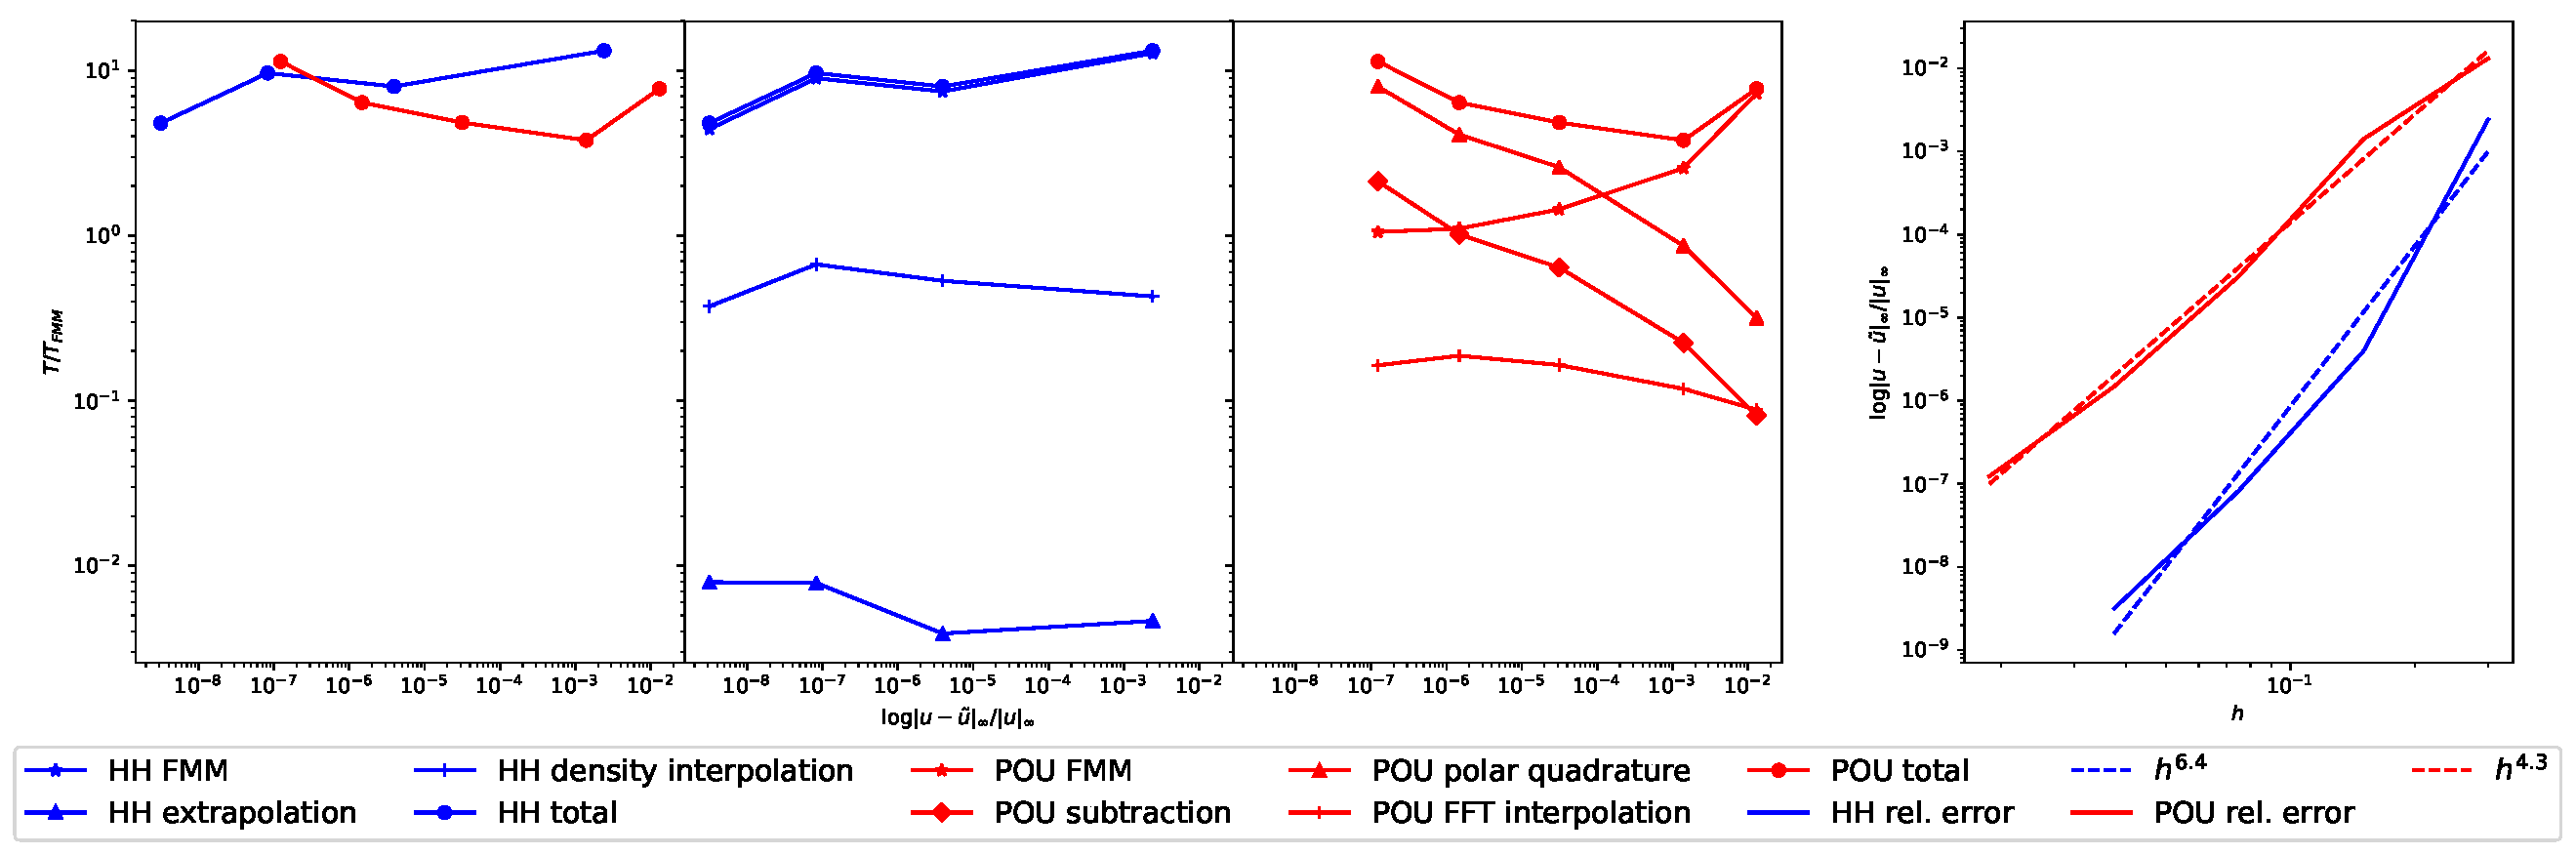
\includegraphics[width=1.2\textwidth]{figs/comparison_cube_laplace_timing.pdf} }

    \makebox[\textwidth][c]{ 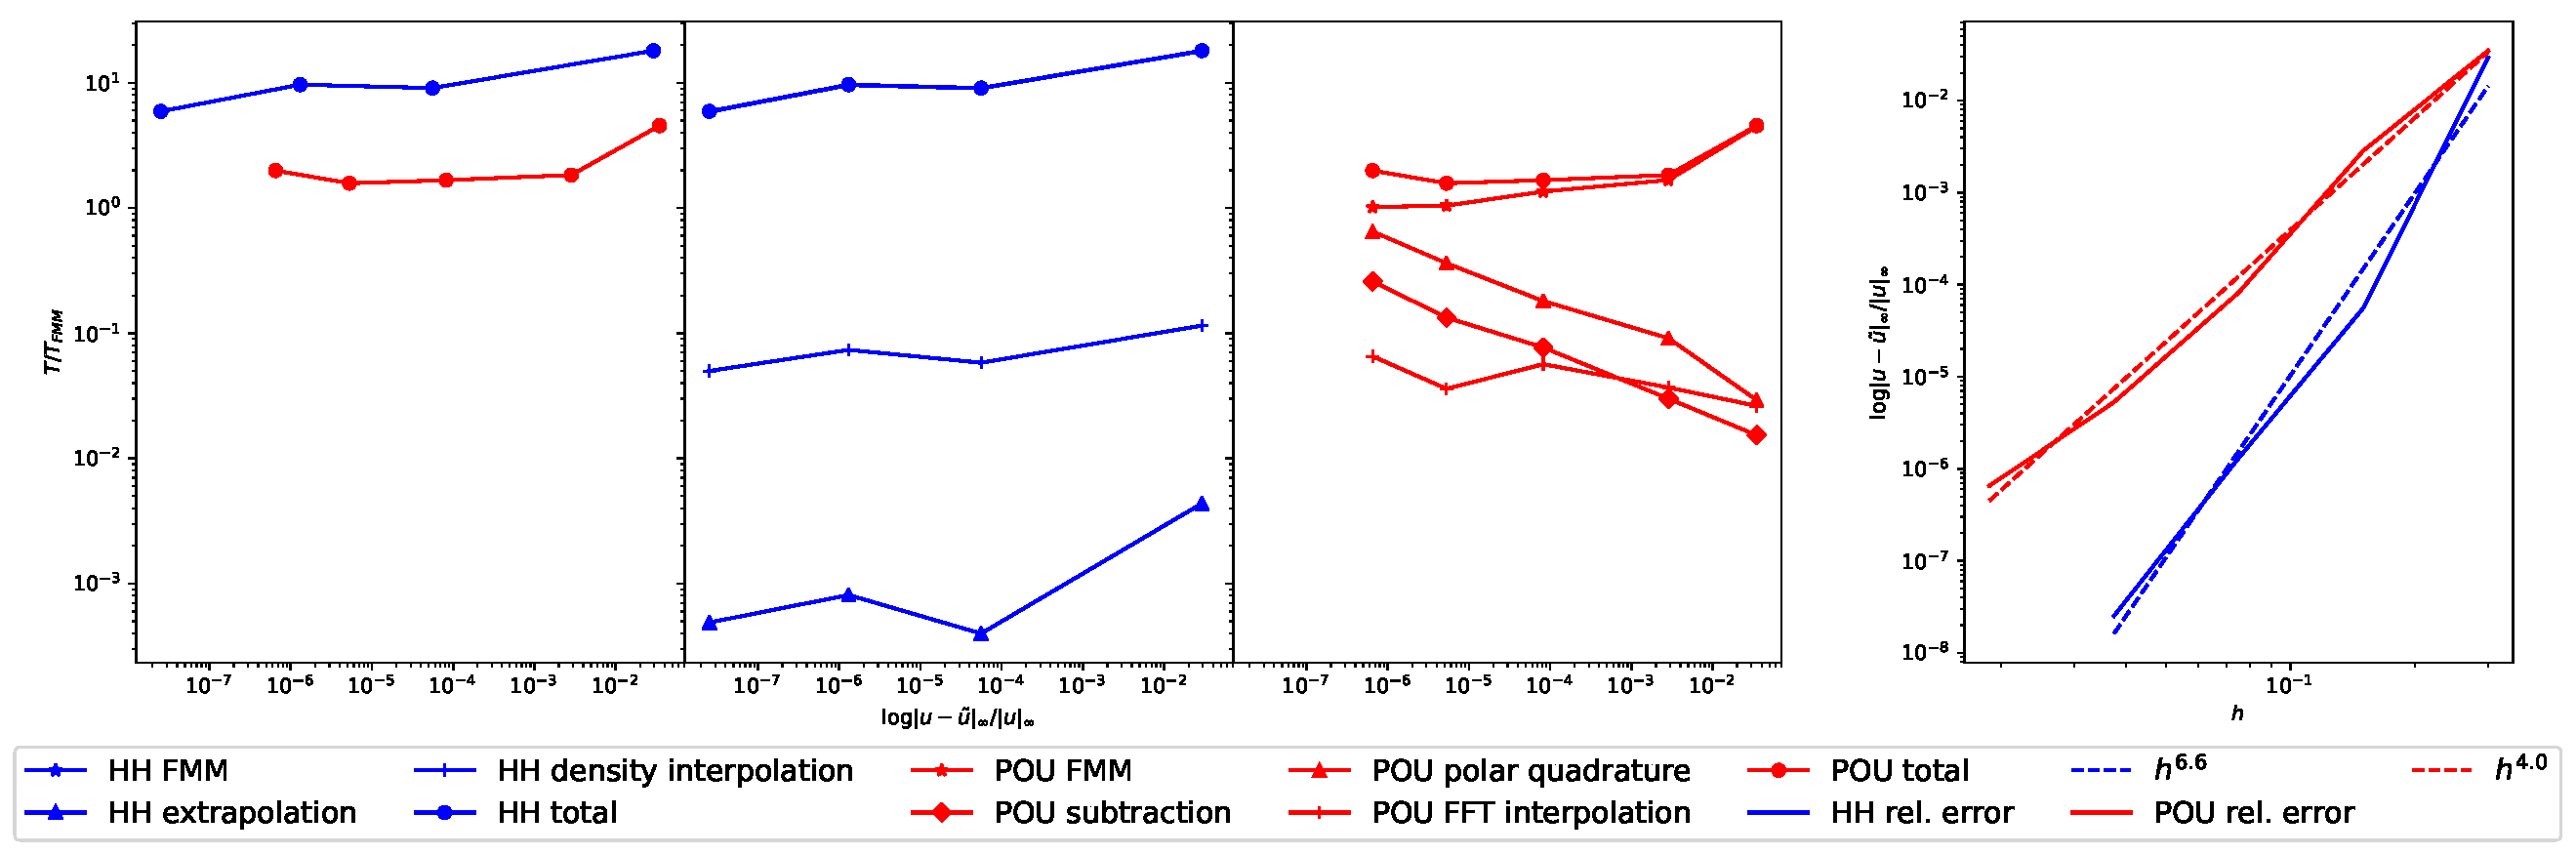
\includegraphics[width=1.2\textwidth]{figs/comparison_cube_const_den_navier_timing.pdf} }
%  \begin{minipage}{\textwidth}
%    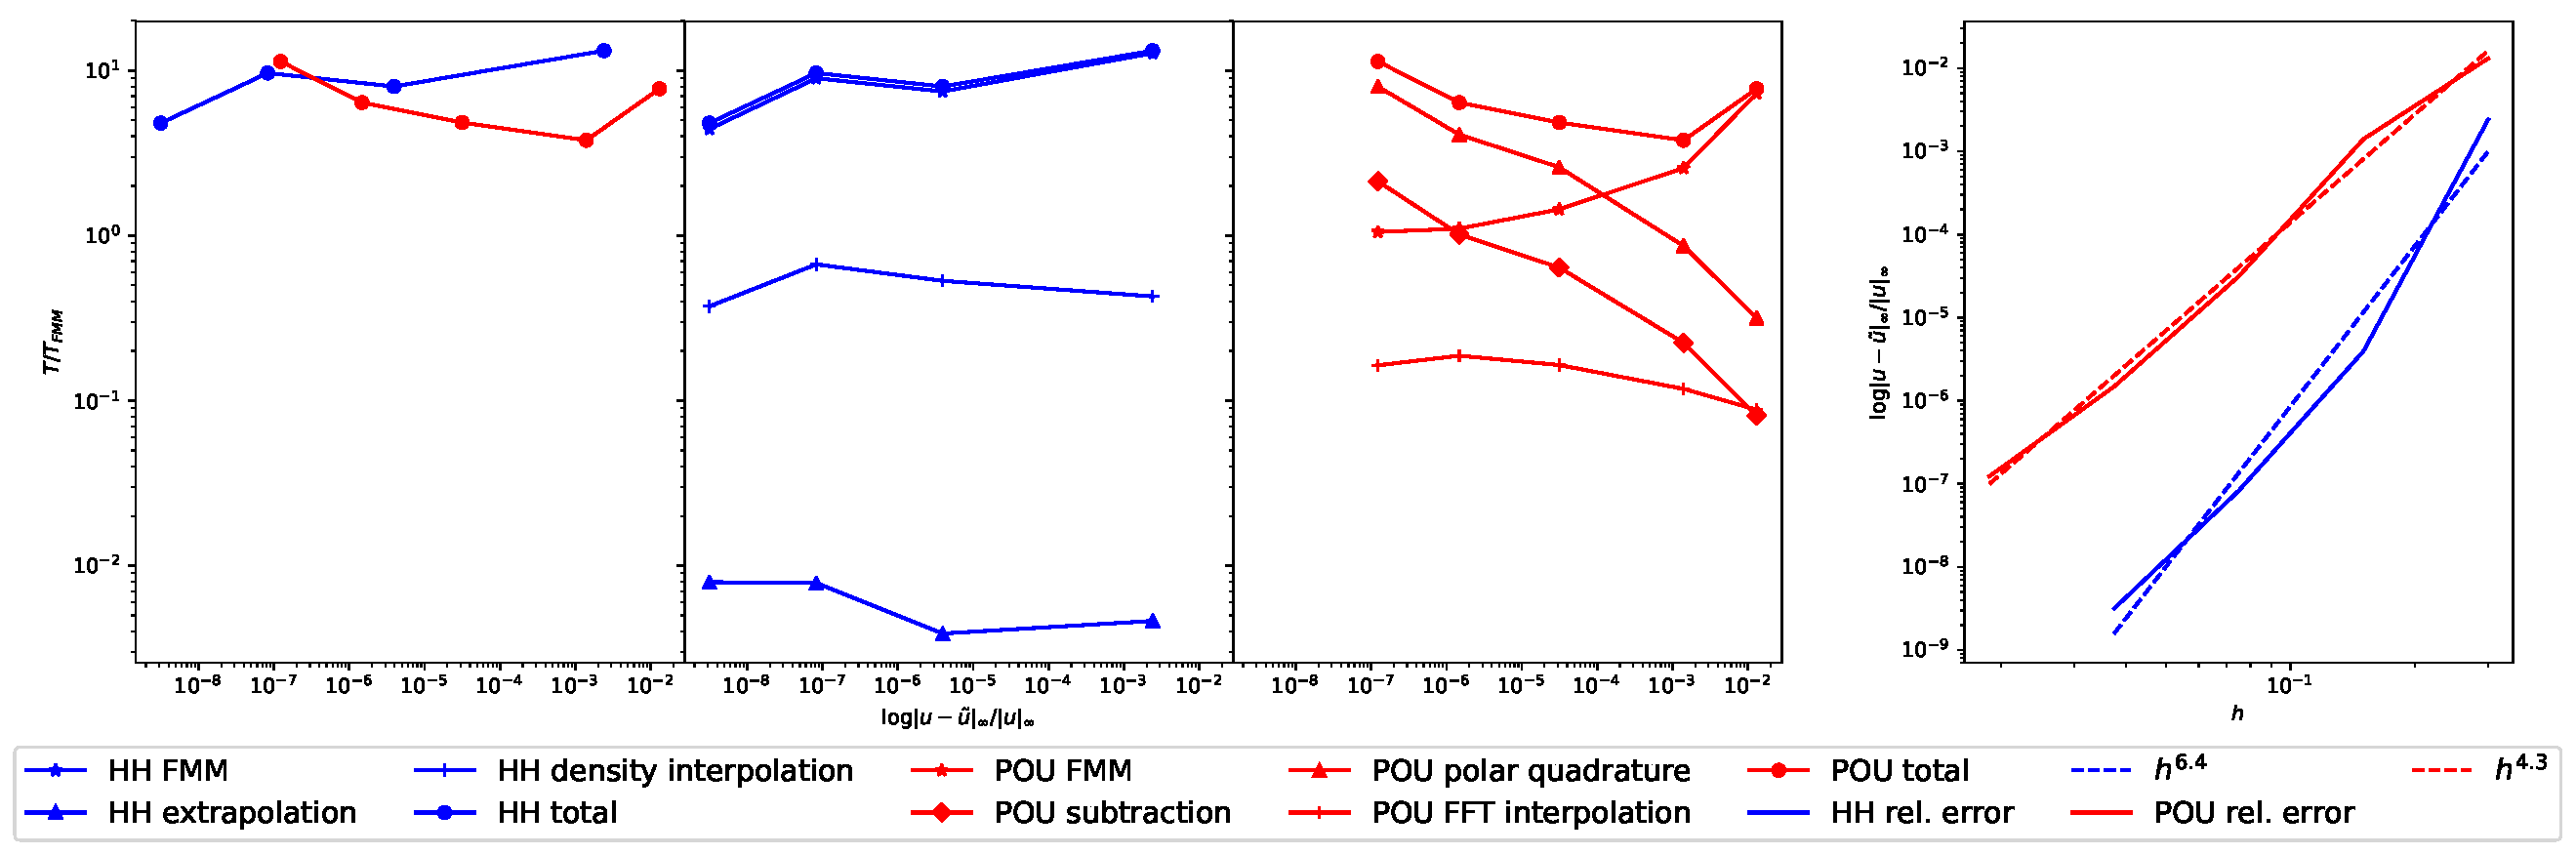
\includegraphics[width=1.5\textwidth]{figs/comparison_cube_laplace_timing.pdf}
%  \end{minipage}\hfill
%  \begin{minipage}{\textwidth}
%    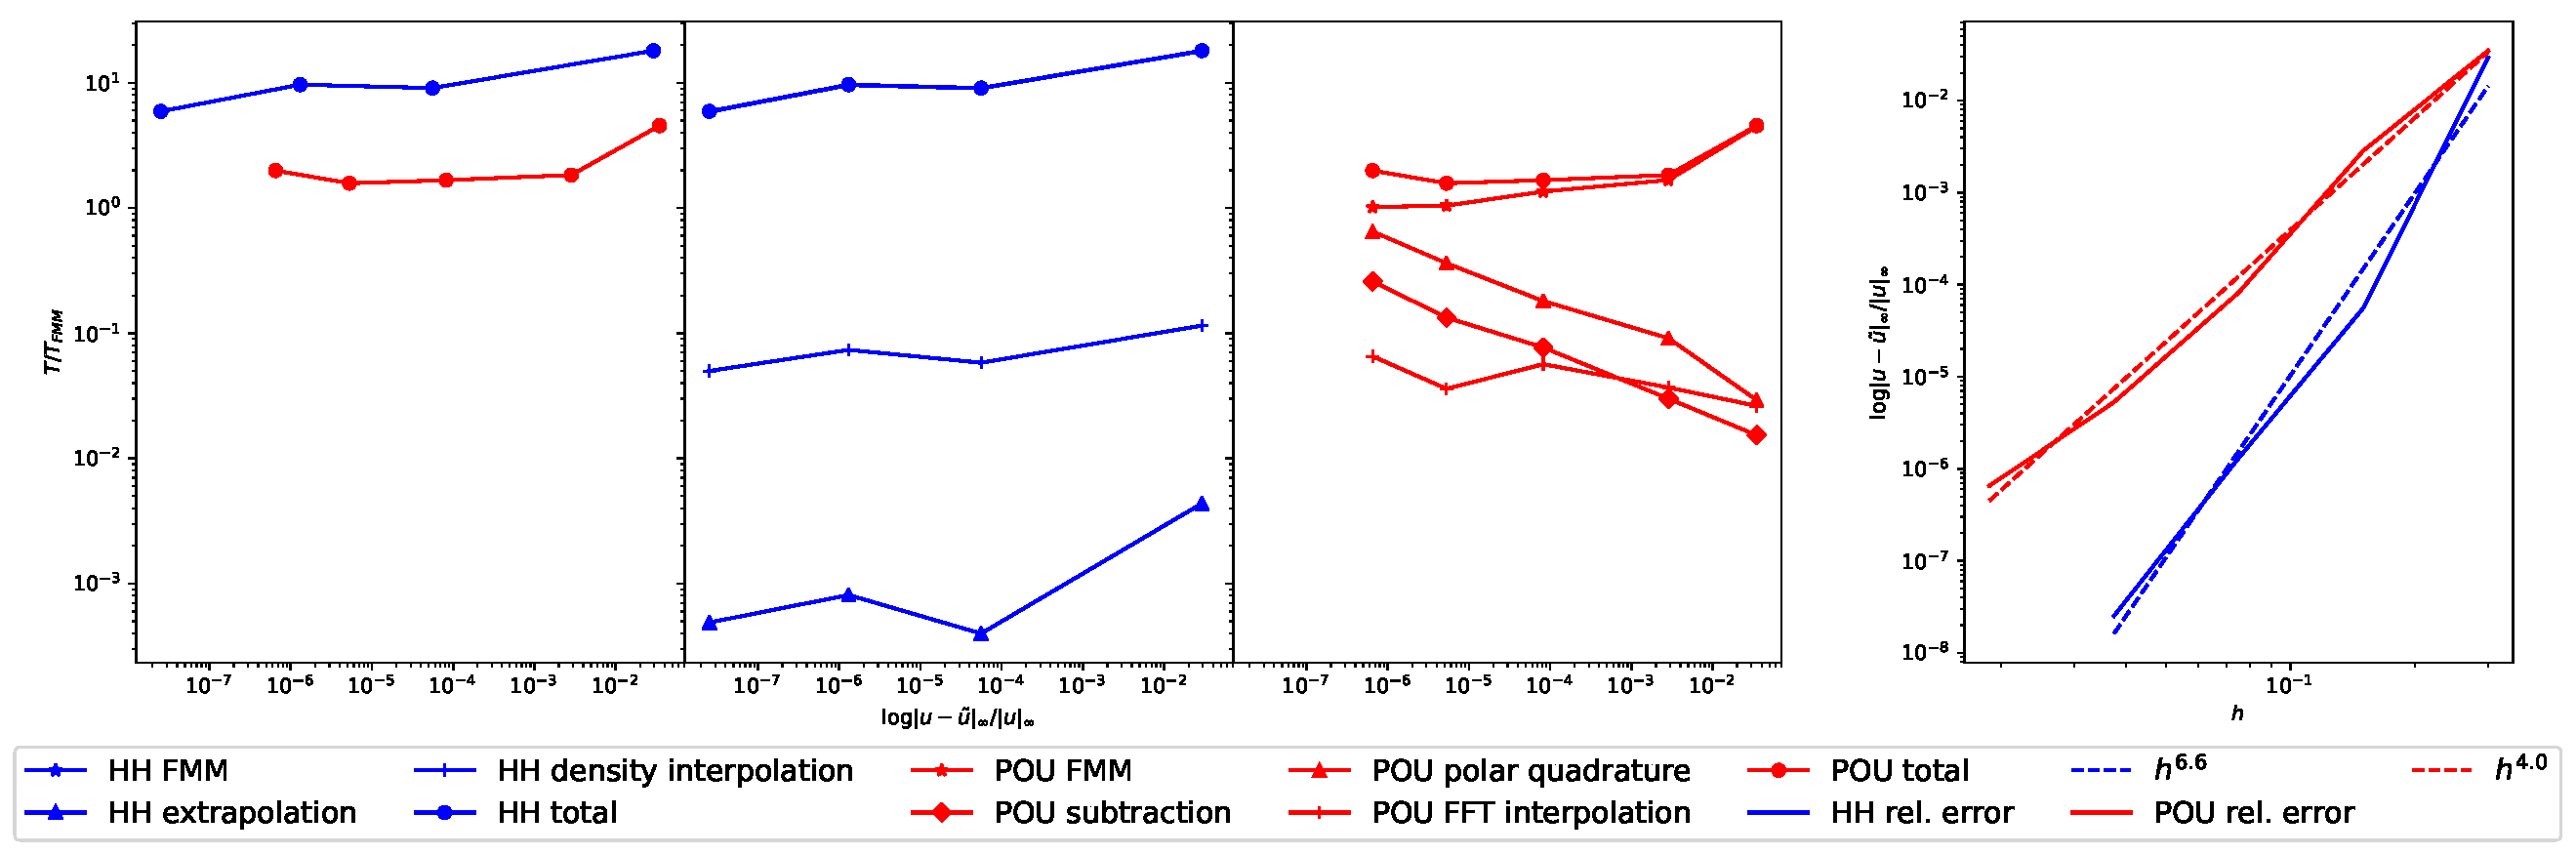
\includegraphics[width=\linewidth]{figs/comparison_cube_const_den_navier_timing.pdf}
%  \end{minipage}\hfill
  \mcaption{fig:compare-const-density}{ Comparison of \qbkix (HH) versus \cite{YBZ}  (POU) on the surface representation of \cite{ying2004simple} evaluating double-layer potential with $\phi=1$}{
      Laplace (top) and elasticity (bottom) problems solved on the sphere shown in \cite[Figure 8-left]{morse2020robust}.
From left to right, we plot the total cost of each scheme, the cost of each subroutine for \qbkix (blue) and the singular quadrature scheme of \cite{YBZ} (red), and the relative error as a function of $h$.
  The plots show the cost and relative error for $h_0 = .3$ representing the right-most data point and each point to the left corresponding to a spacing of $h_i = h_0/2^i$.
For the Laplace problem, we choose $r=.186\sqrt{h}$, $R=1.12\sqrt{h}$ and $p=6$ for \qbkix parameters; for the elasticity problem, we choose $r=.133\sqrt{h}$, $R=.8\sqrt{h}$ and $p=6$. 
The initial spacing parameter is $h_0=.3$.
}
\end{figure}

\begin{figure}[!htb]
  \centering
  \hfill
    \makebox[\textwidth][c]{ 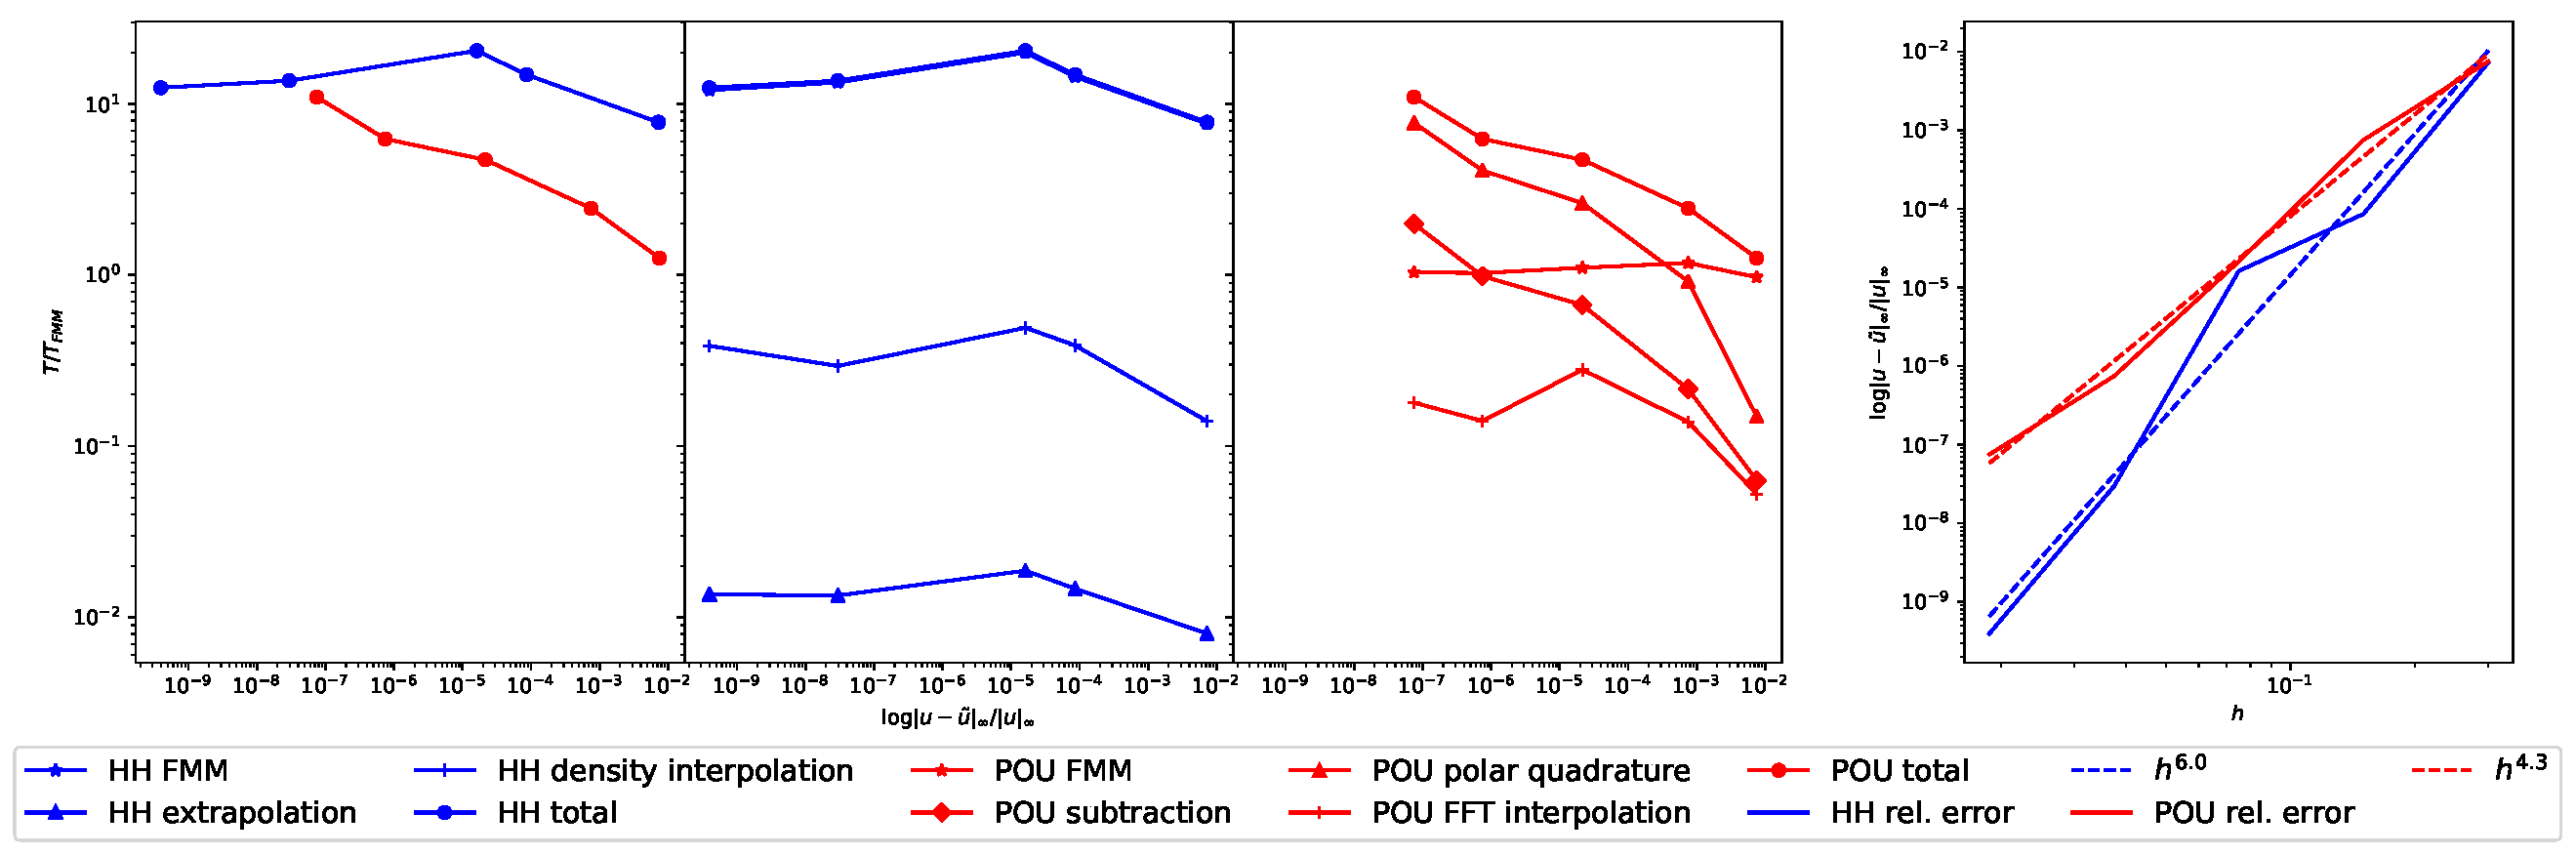
\includegraphics[width=1.2\textwidth]{figs/comparison_cube_solve_laplace_timing.pdf} }
    \makebox[\textwidth][c]{ 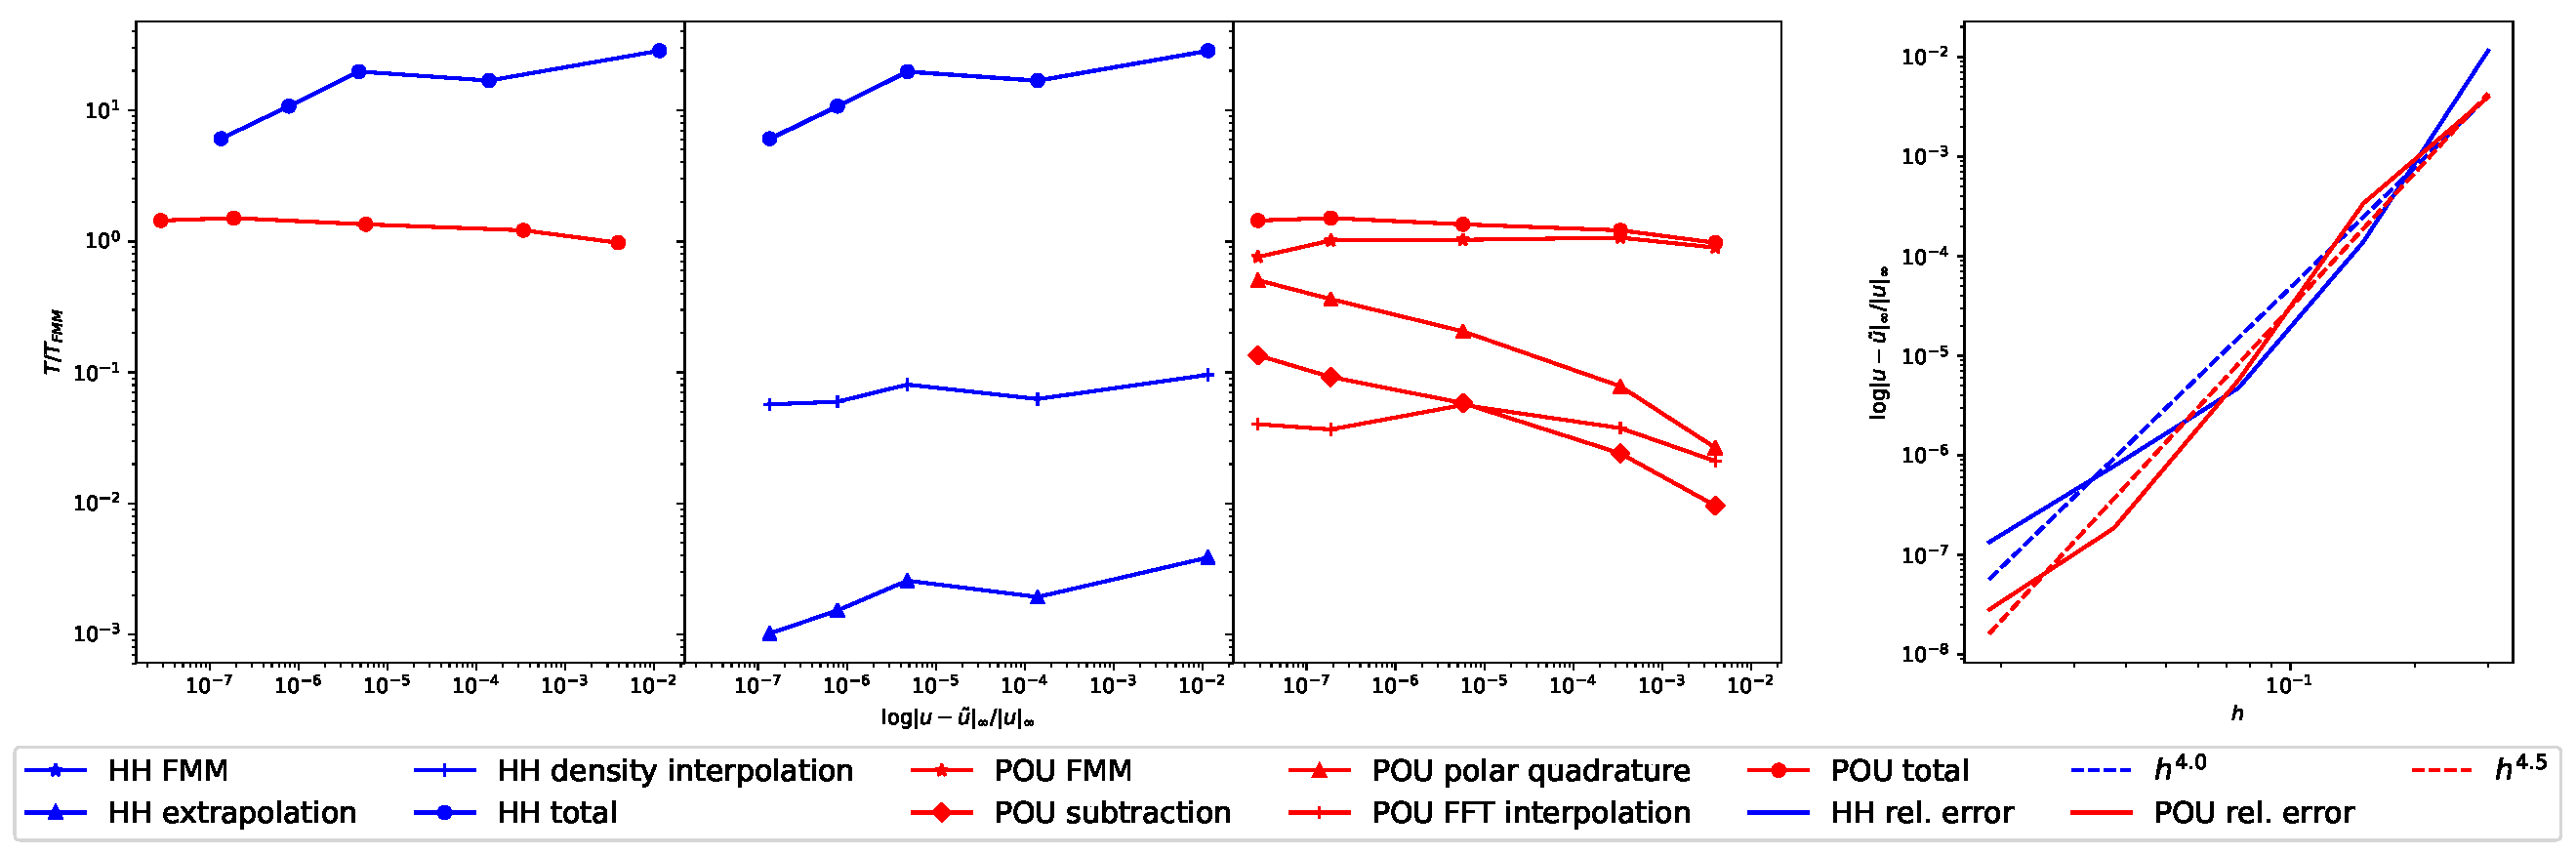
\includegraphics[width=1.2\textwidth]{figs/comparison_cube_navier_timing.pdf} }
%  \begin{minipage}{\textwidth}
%    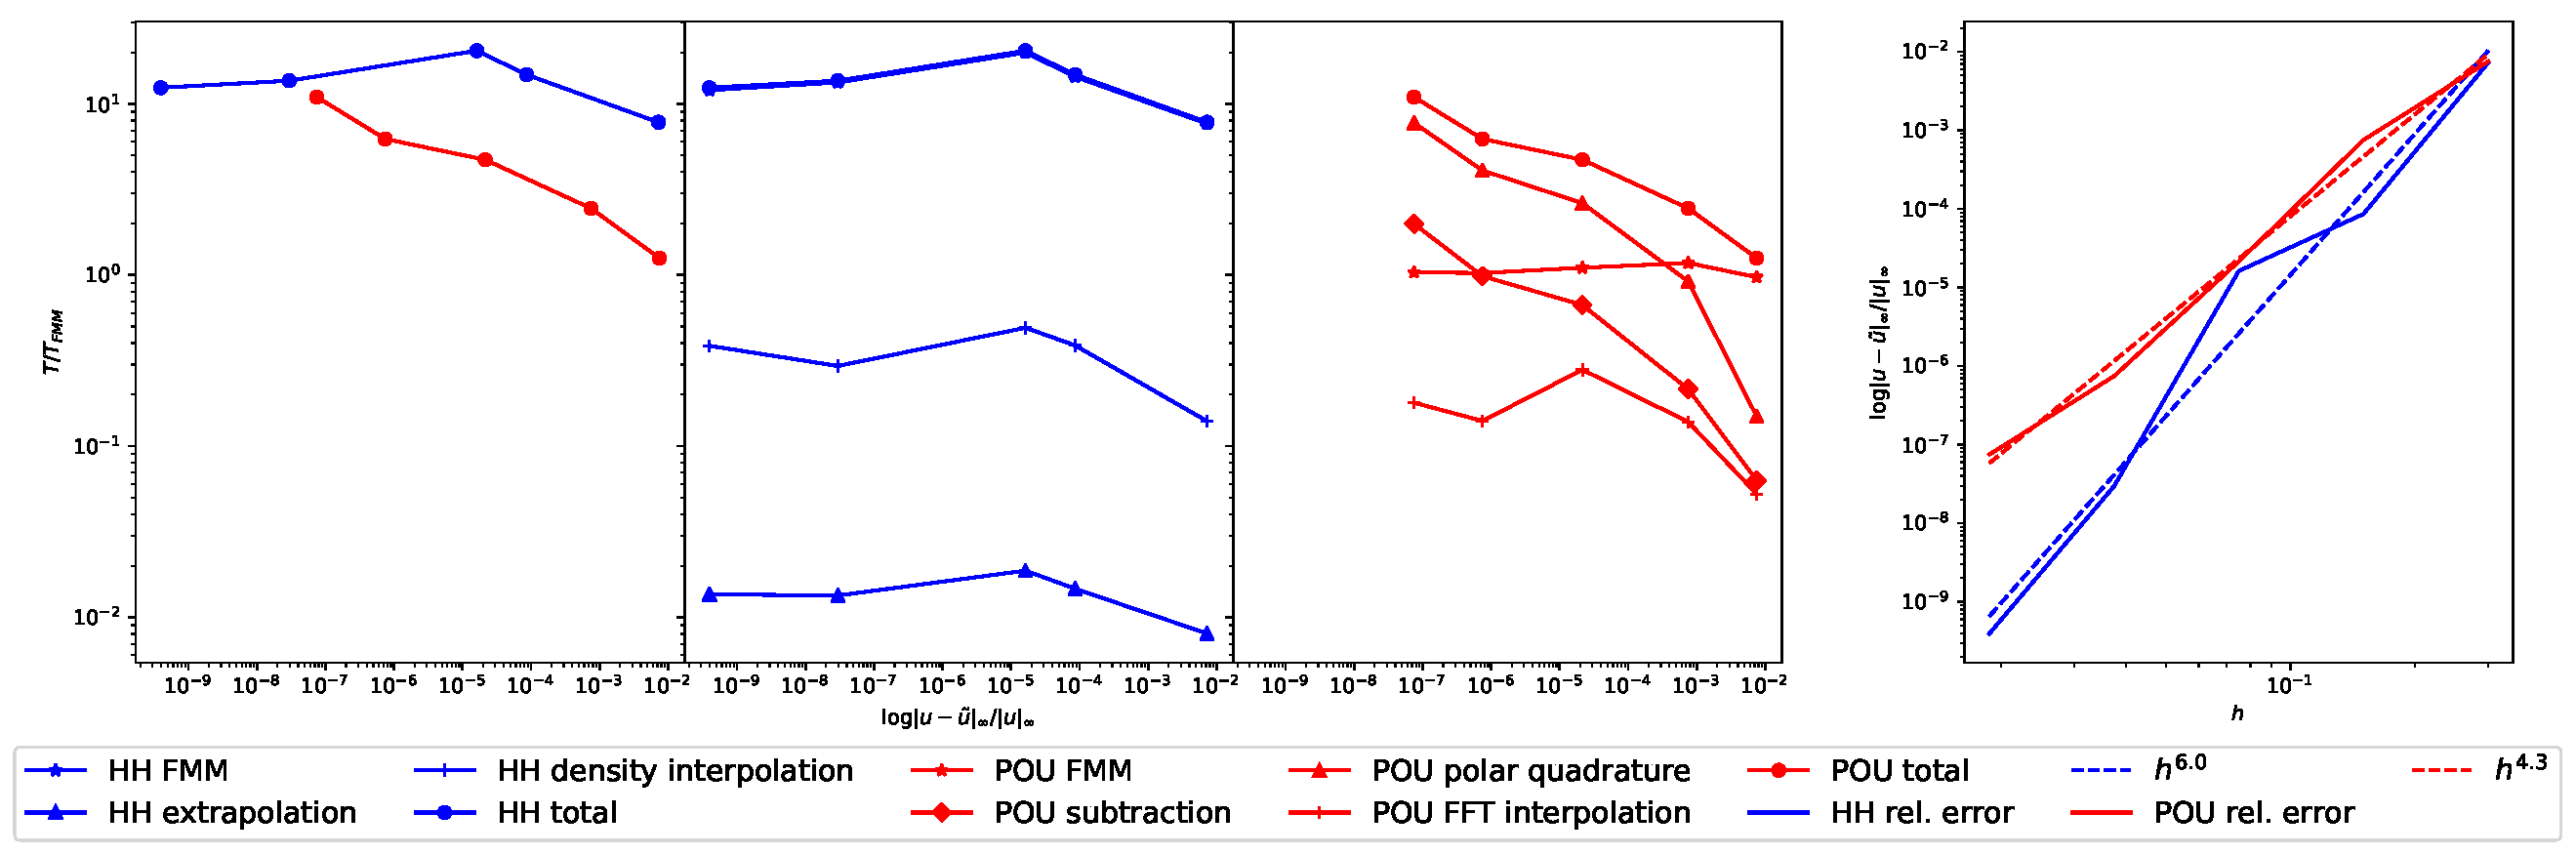
\includegraphics[width=\linewidth]{figs/comparison_cube_solve_laplace_timing.pdf}
%  \end{minipage}\hfill
%  \begin{minipage}{\textwidth}
%    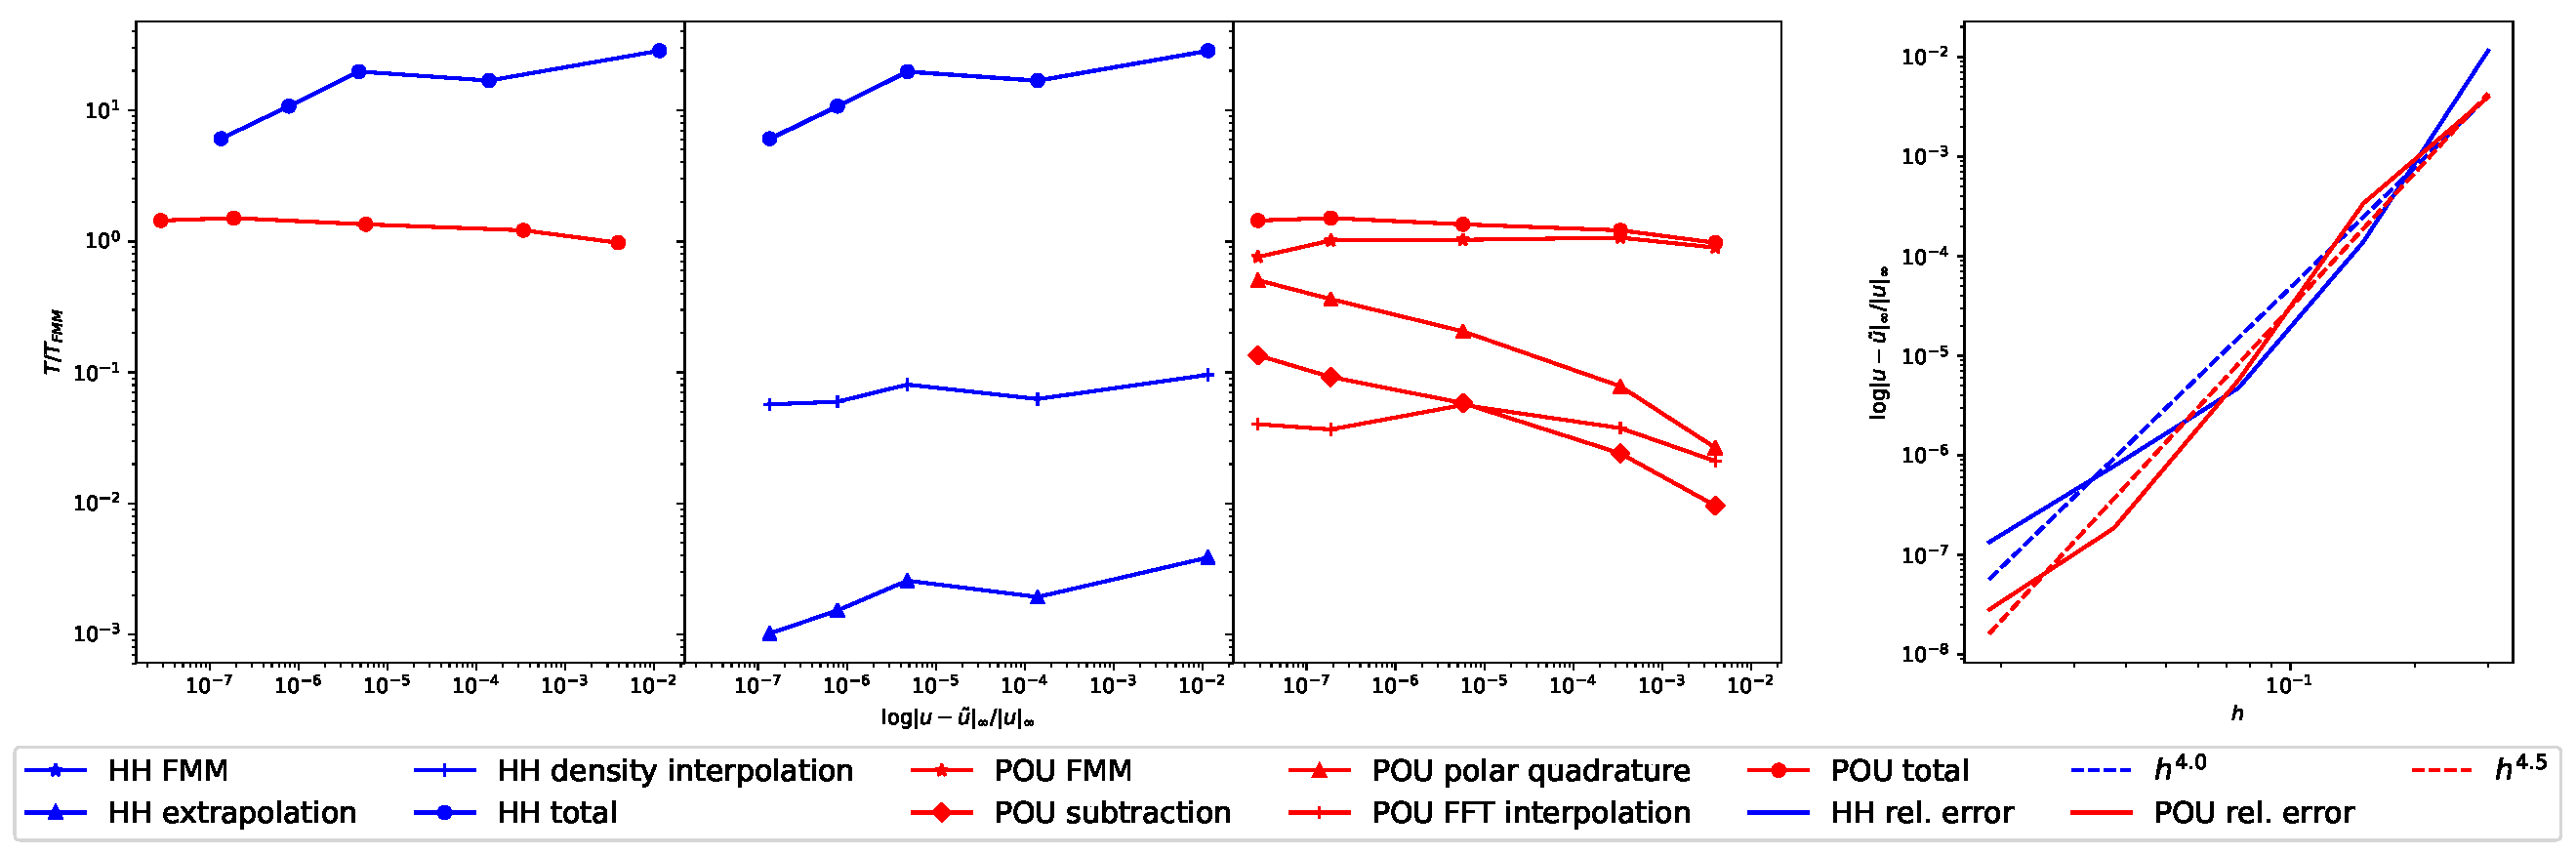
\includegraphics[width=\linewidth]{figs/comparison_cube_navier_timing.pdf}
%  \end{minipage}\hfill
  \mcaption{fig:compare-solve}{Comparison of \qbkix versus \cite{YBZ} on the surface representation of \cite{ying2004simple} solving via \gmres for $u_c$}{
    This figure's format is similar to \cref{fig:compare-const-density}.  
    For the Laplace problem, we choose $r=.028\sqrt{h}$, $R=.172\sqrt{h}$ and $p=6$ for \qbkix parameters; for the elasticity problem, we choose $r=.042\sqrt{h}$, $R=.253\sqrt{h}$ and $p=6$. 
The initial spacing parameter is $h_0=.3$.
  }
\end{figure}

As expected, the \qbkix total cost curves lie somewhere between 1 and 10, since the required \fmm evaluation is $(m+p)$-times larger than $N$.
This step is the dominant cost: the next most expensive step is density interpolation, which is two orders of magnitude faster.
Initially, the main cost of \cite{YBZ} is \fmm evaluation time, but eventually the local correction cost begins to dominant.
Note that the \qbkix and \cite{YBZ}-\fmm curves are not quite flat, due to the initial quadratic complexity of a shallow \fmm tree.

From \cref{fig:compare-const-density,fig:compare-solve}, we observe a higher convergence rate for \qbkix than \cite{YBZ}, except for the elasticity solve in \cref{fig:compare-solve}-bottom where the methods perform about equally.
This allows the cost of \qbkix to decrease below \cite{YBZ} for errors less than $10^{-7}$ for Laplace problems.
More importantly, however, \cite{YBZ} outperforms \qbkix for elasticity problems for all tested discretizations, and also for low and moderate accuracy Laplace problems.
This is due to the greater cost of a vector \fmm evaluation compared to a scalar one: the $m+p$ factor saved in the \fmm evaluation of \cite{YBZ} can be accelerated more efficiently with the method's small dense linear algebra computations.
This means that a local singular quadrature method of \textit{worse} complexity can beat a global method, simply by virtue of reducing the \fmm size.
Moreover, our implementation of \cite{YBZ} is not highly optimized, so we can expect a well-engineered \pou singular quadrature implementation such as \cite{malhotra2019taylor} to widen this gap.
By noting the large difference between the \qbkix \fmm cost and the \qbkix density interpolation, we can reasonably infer that a local \qbkix scheme should narrow this gap and outperform \cite{YBZ}, assuming that this transition does not dramatically affect error convergence.
%%%%%%%%%%%%%%%%%%%%%%%%%%%%%%%%%%%%%%%%%%%%%%%%%%%%%%%%%%%%%%%%%%%%%%%%%%%%%%%
%%% Cut ending here
%%%%%%%%%%%%%%%%%%%%%%%%%%%%%%%%%%%%%%%%%%%%%%%%%%%%%%%%%%%%%%%%%%%%%%%%%%%%%%%
\iffalse
%\paragraph{Comparison on approximate polynomial surfaces}
To compare the full \qbkix method with \cite{YBZ}, we fit polynomial patches to the $C^\infty$ surface of \cite{ying2004simple}, denoted $\Gamma_b$, to produce $\Gammah$ during the first step of \cref{sec:admissible_algo}.
We then apply the remaining geometry preprocessing algorithms of \cref{sec:admissible_algo} to $\Gammah$ to produce $\Pcoarse$.
After producing $\Pfine$ with two levels of uniform upsampling, we solve \cref{eq:int-eq} with two-sided \qbkix on $\Gammah$ and evaluate the solution on the boundary with one-sided \qbkix.
We then solve for the solution to \cref{eq:int-eq} on $\Gamma_b$ using \cite{YBZ}. 

For each of the tests in this section, we choose some initial spacing parameter $h_0$ to discretize the surface of \cite{ying2004simple} as in \cite{YBZ} and use the same $16\times$ upsampled grid and floating partition of unity size of size $O(\sqrt{h})$ as in \cite{YBZ}.
We apply \qbkix to $\Gammah$ and the scheme of \cite{YBZ} to $\Gamma_b$ with spacing $h_0$ and compute the relative error and collect timing statistics for the important components of each method.
We repeat this test with $h_0/2^i$ for \cite{YBZ} and $i$ levels of subdivision in $\Pcoarse$ for $i=1,\hdots 4$ and plot the results.

As in the previous section, we choose the parameters $r$ and $R$ of \qbkix to be $O(\sqrt{L})$ to observe standard convergence behavior.
For both quadrature methods, we use a multipole order of $16$ for \pvfmm with at most 250 points in each leaf box.
\begin{figure}[!htb]
  \centering
    \makebox[\textwidth][c]{ 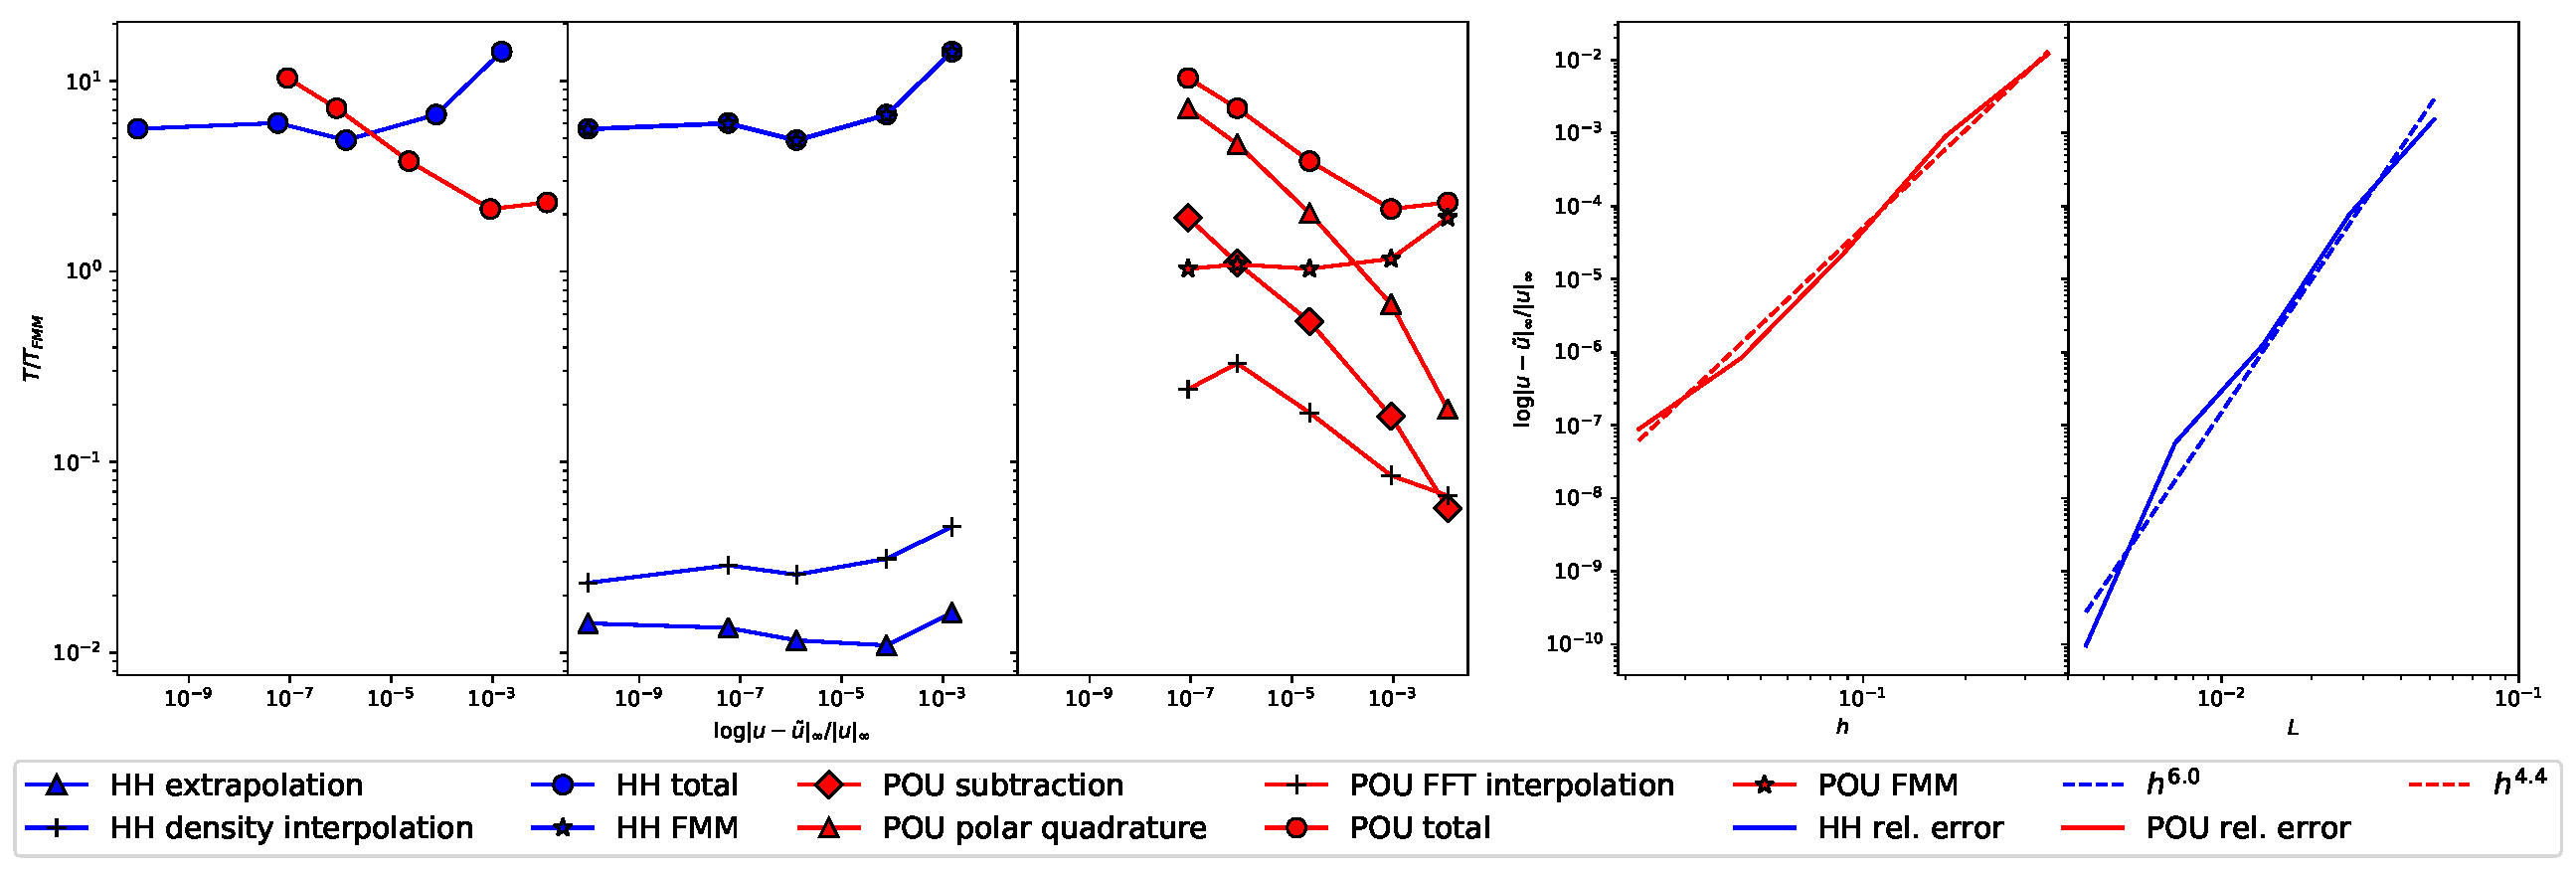
\includegraphics[width=1.\textwidth]{figs/comparison_face_map_vs_blendsurf_cube_laplace_timing.pdf} }
    \makebox[\textwidth][c]{ 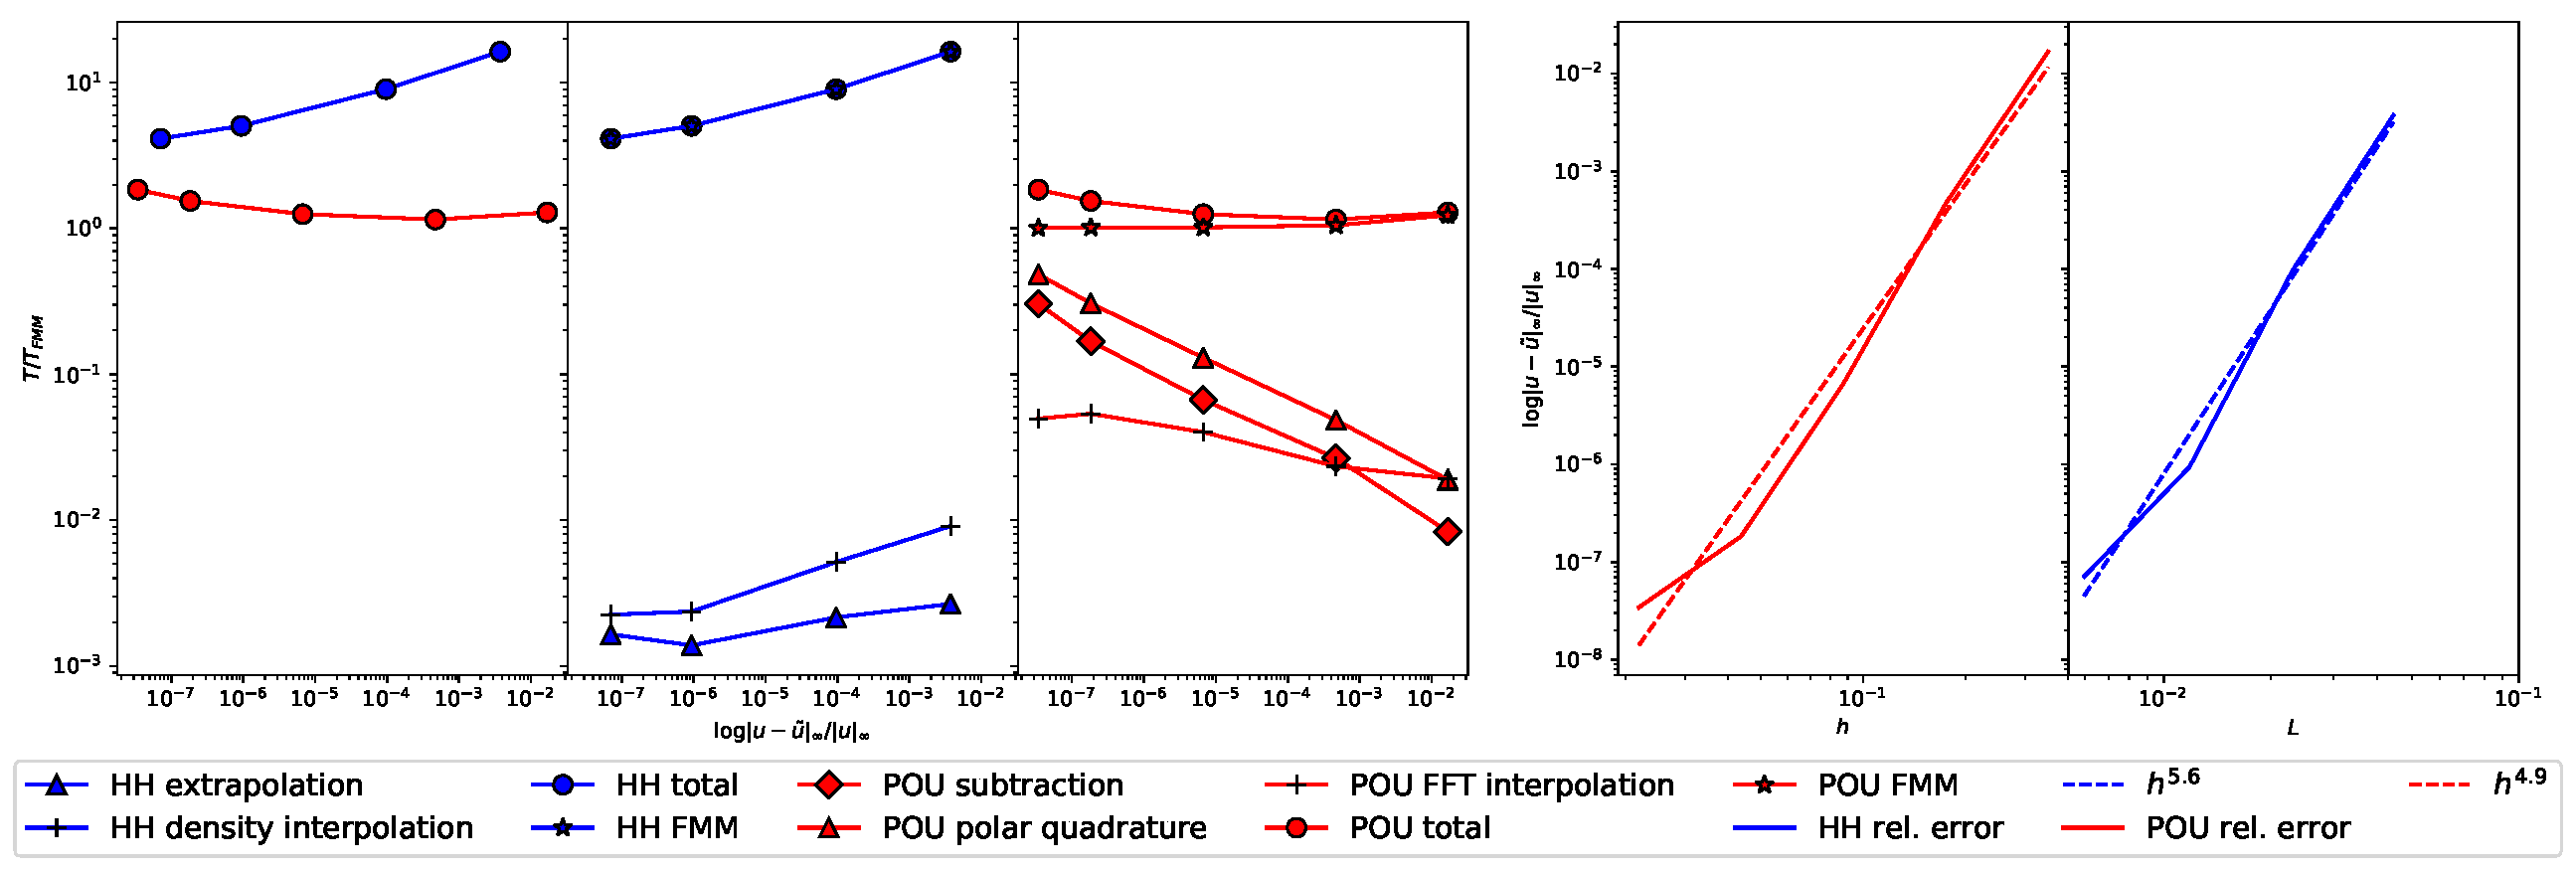
\includegraphics[width=1.\textwidth]{figs/comparison_face_map_vs_blendsurf_cube_navier_timing.pdf} }
%  \hfill
%  \begin{minipage}{\textwidth}
%    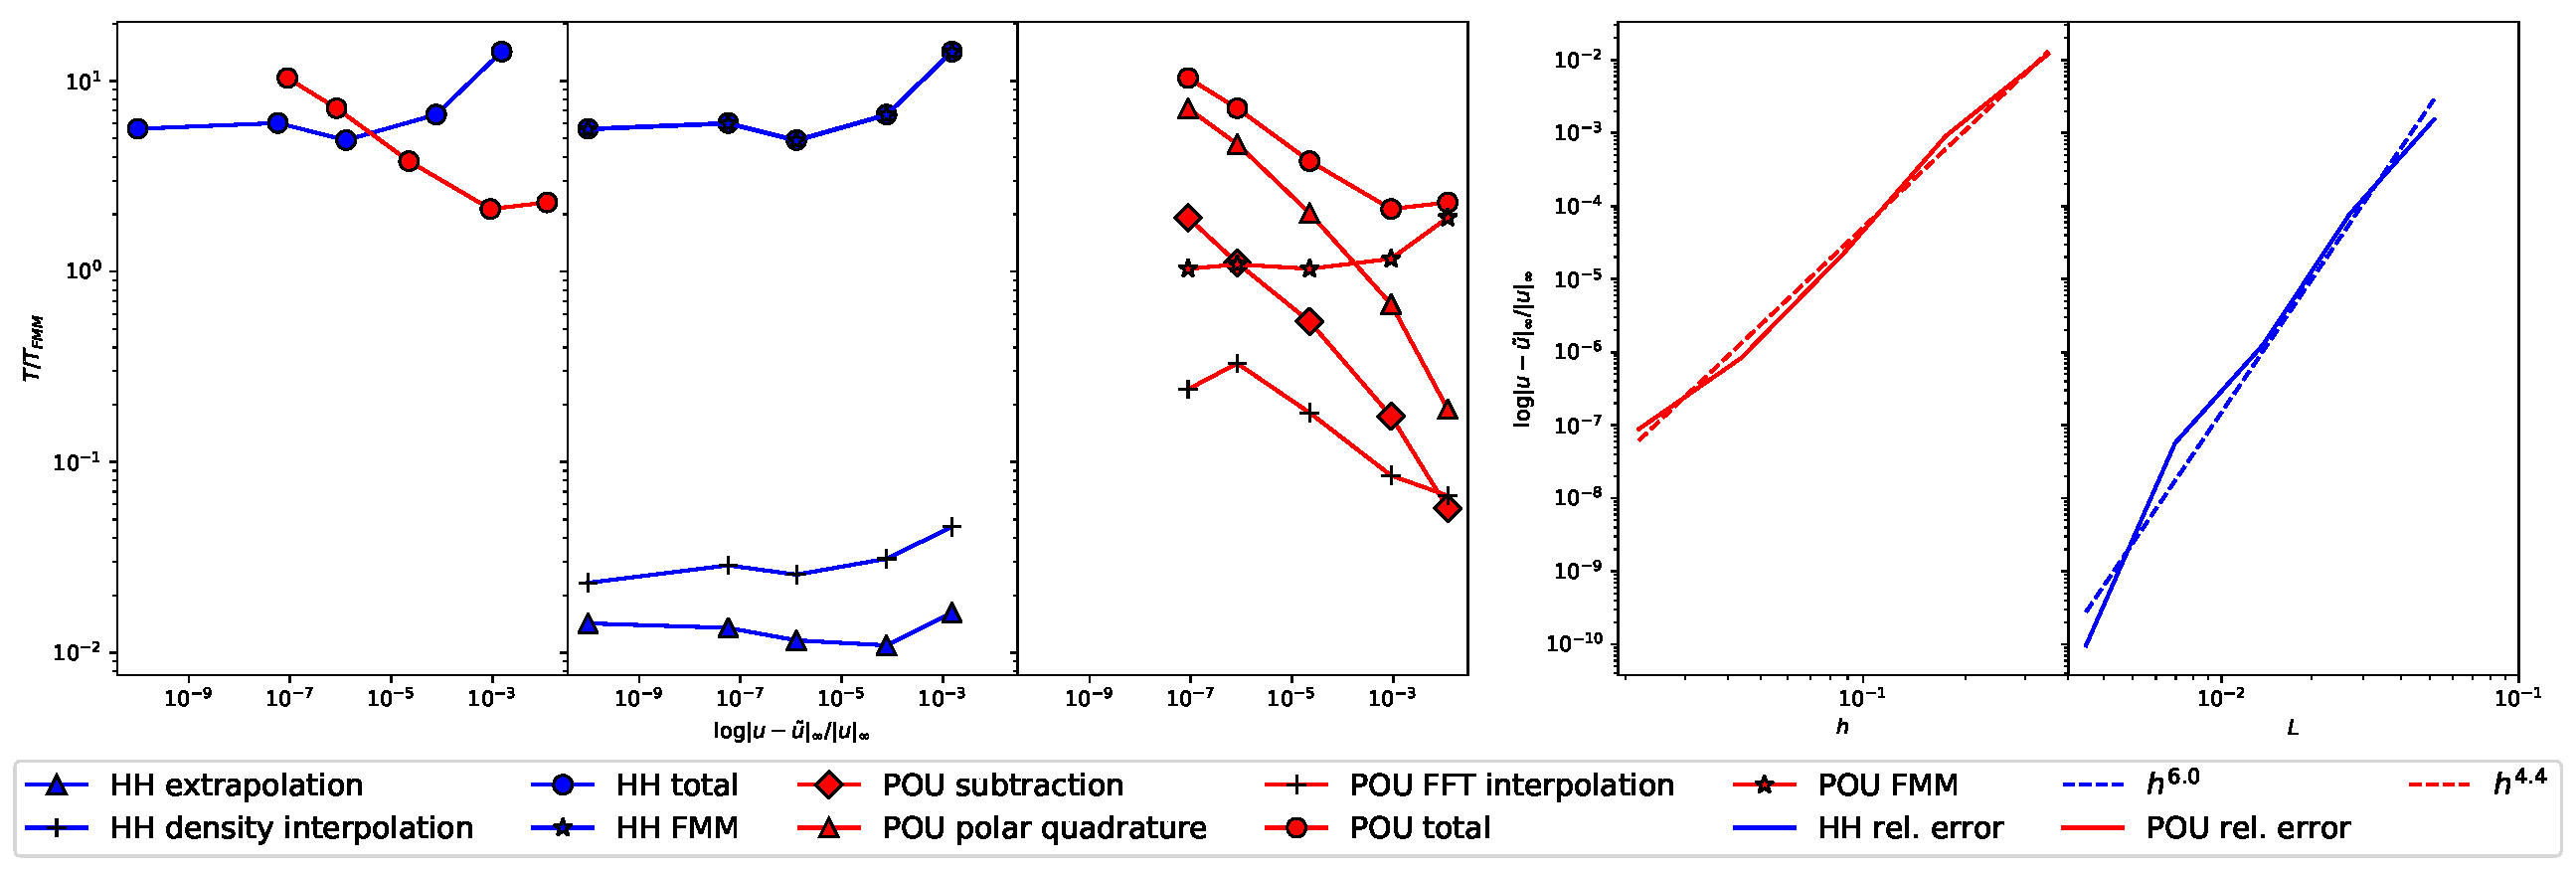
\includegraphics[width=\linewidth]{figs/comparison_face_map_vs_blendsurf_cube_laplace_timing.pdf}
%  \end{minipage}\hfill
%  \begin{minipage}{\textwidth}
%    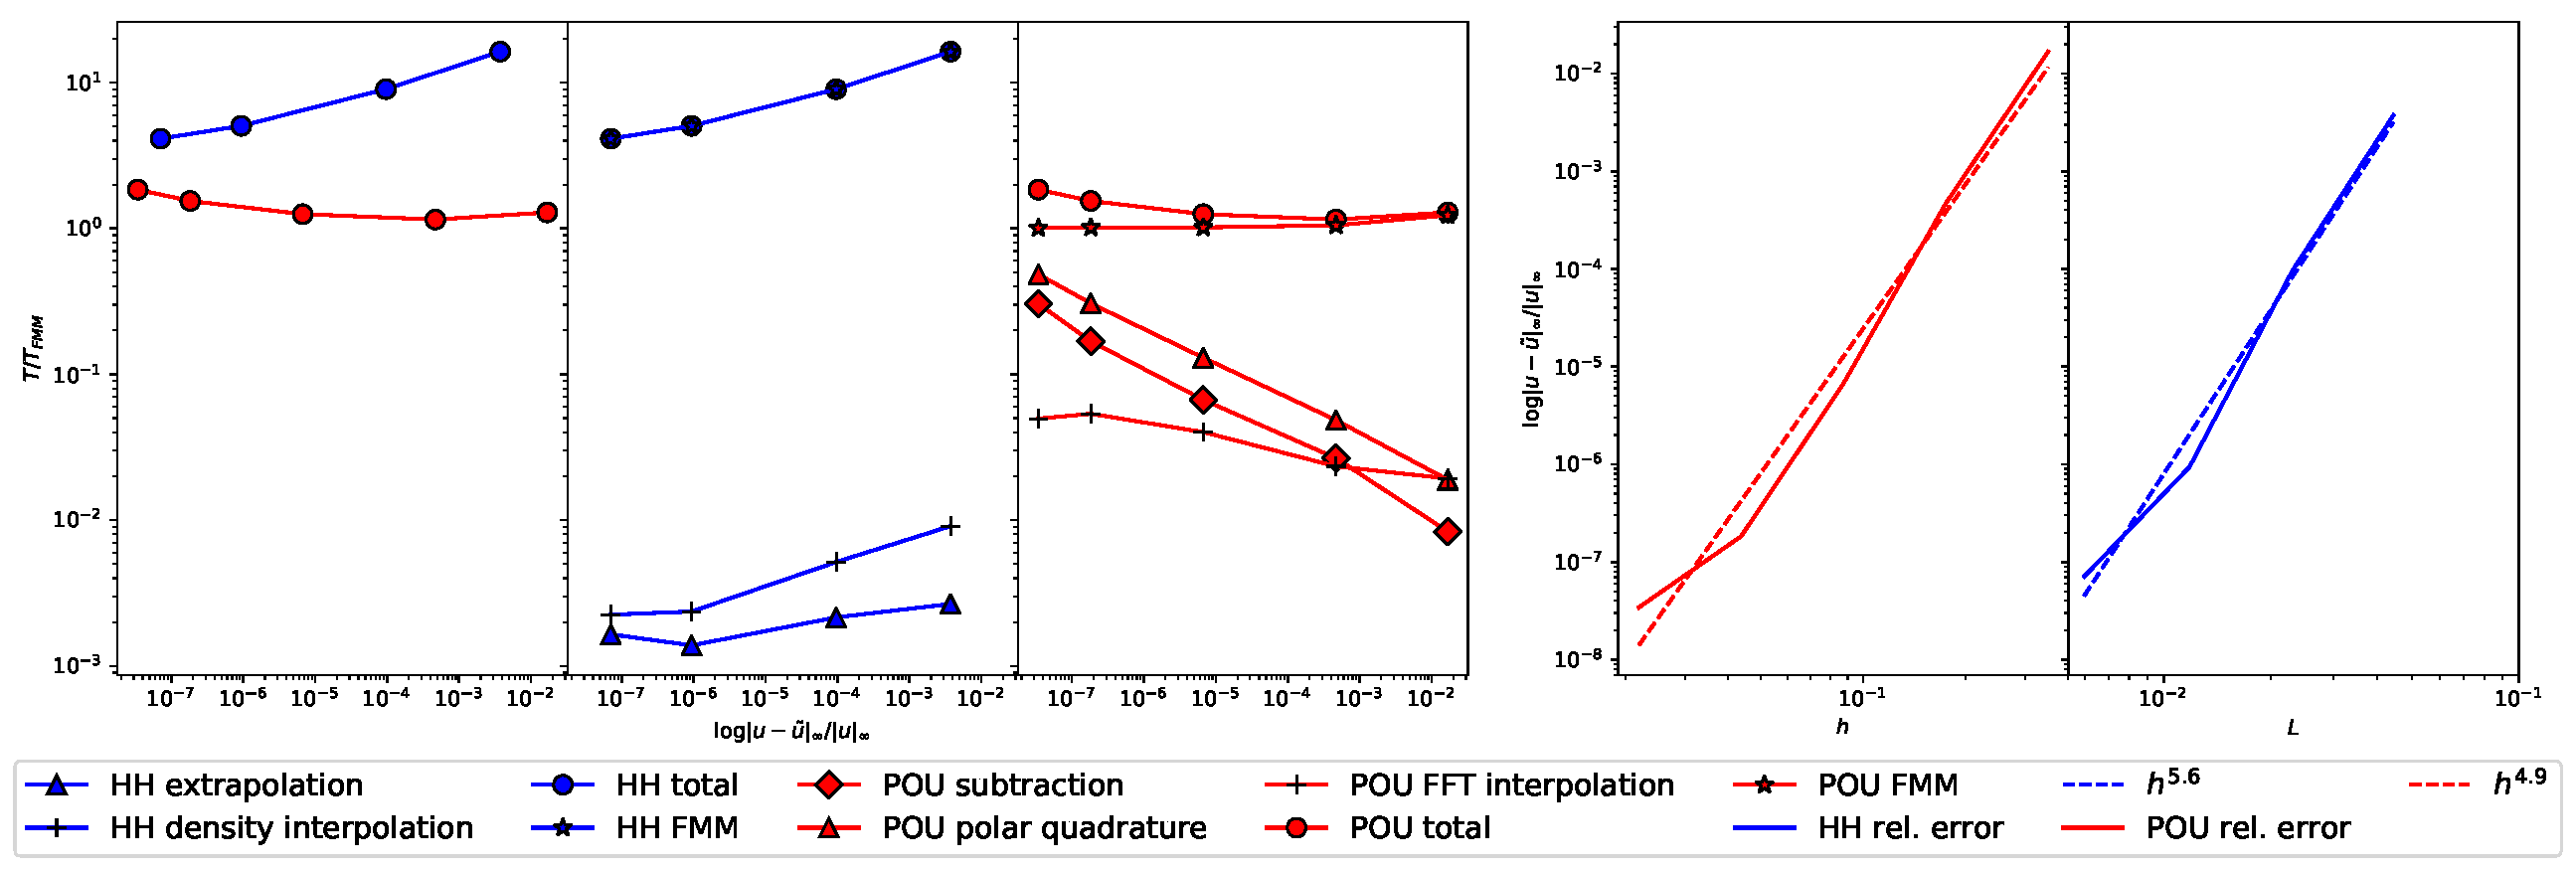
\includegraphics[width=\linewidth]{figs/comparison_face_map_vs_blendsurf_cube_navier_timing.pdf}
%  \end{minipage}\hfill
    \mcaption{fig:compare-solve-surface}{Comparison of \qbkix on polynomial patches (HH) versus \cite{YBZ} on the surface representation of \cite{ying2004simple} (POU) solving via \gmres for $u_c$}{
    Laplace (top) and elasticity (bottom) problems solved on the sphere shown in \cref{fig:greens-id-test-cases}.
From left to right, we plot the total cost of each scheme, the cost of each subroutine for \qbkix (blue) and the singular quadrature scheme of \cite{YBZ} (red), and the relative error as a function of $h$.
    We plot error convergence of \cite{YBZ} as a function of $h$ and \qbkix as a function of $L$, due to the distinct discretizations.
    For \qbkix parameters, we choose $r=.013\sqrt{L}$, $R=.075\sqrt{L}$ for the Laplace problem; for the elasticity problem, we choose $r=.013\sqrt{L}$, $R=.08\sqrt{L}$. We choose $p=6$ and $q=15$ for both problems.
    For \cite{YBZ} the spacing is $h_0=.35$.
  }
\end{figure}
The results are shown in \cref{fig:compare-solve-surface}. 
From left to right, each plot details the total cost of each scheme, the cost of each subroutine for \qbkix (denoted \abbrev{HH}) and the singular quadrature scheme of \cite{YBZ} (denoted \abbrev{POU}), and the relative error as a function of $h$ and $L$, respectively.
Each data point in the plots, from right to left, is the result of $4\times $ finer sampling of the surfaces.
We plot the cost of both schemes the cost of each algorithmic step as a function of their computed relative error. 
In each figure, we present results for a Laplace problem (top) and an elasticity problem (bottom), to highlight the difference in performance between scalar and vector kernels.

From \cref{fig:compare-solve-surface}, we observe a slightly higher convergence rate for \qbkix than \cite{YBZ}, which is consistent with original results.
More importantly, however, \cite{YBZ} outperforms \qbkix for elasticity problems for all tested discretizations, and also for low and moderate accuracy Laplace problems.
This is due to the greater cost of a vector \fmm evaluation compared to a scalar one: the $m+p$ factor saved in the \fmm evaluation of \cite{YBZ} can be accelerated more efficiently with the method's small dense linear algebra computations.
This means that a local singular quadrature method of \textit{worse} complexity can beat a global method, simply by virtue of reducing the \fmm size; we observe that the \fmm evaluation in \cref{fig:compare-solve-surface} accounts for at least 95\% of the \qbkix cost.
Moreover, our implementation of \cite{YBZ} is not highly optimized, so we can expect a well-engineered \pou singular quadrature implementation such as \cite{malhotra2019taylor} to widen this gap.
By noting the large difference between the \qbkix \fmm cost and the \qbkix density interpolation, we can reasonably infer that a local \qbkix scheme should narrow this gap and outperform \cite{YBZ}, assuming that this transition does not dramatically affect error convergence.

%\qbkix is more efficient in the high-accuracy regime for Laplace problems, but \cite{YBZ} is more efficient for low-accuracy Laplace and elasticity problems.
%However, main difference from the previous section is that the crossover point in performance appears to be larger; \qbkix becomes more efficient than \cite{YBZ} around $10^{-5}$ and the gap between \qbkix and \cite{YBZ} for elasticity is less dramatic at $10^{-8}$.
%We attribute this improvement to the more efficient Clenshaw-Curtis discretization of \qbkix compared to the overlapping trapezoidal discretization of \cite{YBZ}.
%This is further supporting evidence that a local \qbkix implementation should surpass \cite{YBZ}.
\subsection{Requested target precision vs. computed accuracy}
\begin{figure}[!htb]
\begin{tikzpicture}
    \begin{loglogaxis}[
        xlabel=$\err{target}$,
        ylabel= $\infty$-norm relative error,
        ylabel near ticks,
        xlabel near ticks,
        label style={font=\scriptsize},
        tick label style={font=\scriptsize},
        width=.333\linewidth%7cm,height=3cm
    ]
    \addplot[smooth,mark=*,blue] plot coordinates {
        (1e-4,0.0003143683435301948)
        (1e-5,6.031924968205908e-05)
        (1e-6,4.103514547039301e-06)
        (1e-7,6.614064613404895e-07)
        (1e-8,1.122384348756594e-07)
    };
        \addplot[domain=1e-8:1e-4,dotted,thick]{x};

    \end{loglogaxis}
    \end{tikzpicture}
    \begin{tikzpicture}
    \begin{semilogxaxis}[
        xlabel=$\err{target}$,
        ylabel= Target points/second/core,
        ylabel near ticks,
        xlabel near ticks,
        label style={font=\scriptsize},
        tick label style={font=\scriptsize},
        width=.333\linewidth%7cm,height=3cm
    ]
    \addplot[smooth,mark=*,blue] plot coordinates {
        (1e-4,2077)
        (1e-5,1620)
        (1e-6,772)
        (1e-7,400)
        (1e-8,222)
    };
    \end{semilogxaxis}
    \end{tikzpicture}
    \begin{tikzpicture}
    \begin{loglogaxis}[
        xlabel=$\err{target}$,
        ylabel= Number of patches,
        ylabel near ticks,
        xlabel near ticks,
        label style={font=\scriptsize},
        tick label style={font=\scriptsize},
        legend style={font=\tiny},
         legend image post style={scale=0.5},
        width=.333\linewidth%7cm,height=3cm
    ]
    \addplot[smooth,mark=*,blue] plot coordinates {
        (1e-4,128)
        (1e-5,128)
        (1e-6,128)
        (1e-7,128)
        (1e-8,128)
    };
    \addlegendentry{$|\Pcoarse|$}
    \addplot[smooth,mark=*,red] plot coordinates {
        (1e-4,5408)
        (1e-5,8288)
        (1e-6,28256)
        (1e-7,60032)
        (1e-8,113936)
    };
    \addlegendentry{$|\Pfine|$}
    \end{loglogaxis}
    \end{tikzpicture}
        \mcaption{fig:full-algo-perf}{Performance of full algorithm}{
            Left: $\infty$-norm relative error in singular integral vs requested target accuracy (blue). 
        The dotted line is the ideal behavior $y=x$.
        Middle: Performance in terms of target points evaluated per second per core with \qbkix.
        Right: Number of patches in $\Pcoarse$ and $\Pfine$ computed by the preprocessing algorithms.}
\end{figure}

In this section, we study the performance of the full algorithm outlined in \cref{sec:algo}.
We test \qbkix on the torus domain shown in \cref{fig:greens-id-test-cases}-right.
We choose a reference solution of the form of \cref{eq:point-charge-solution} with a single point charge located at the origin, in the middle of the hole of the torus.
We solve the integral equation with two-sided \qbkix and evaluate the singular integral on a distinct discretization with one-sided \qbkix.
We choose $q=20$, $p=6$ and $a=b/6$.
We select various values for $\err{target}$ using the plot in \cref{fig:extrap-err-p6} to choose $b$ to ensure sufficiently accurate extrapolation. 
We plot the results of our tests in \cref{fig:full-algo-perf}.

We see in \cref{fig:full-algo-perf}-left that we are consistently close to the requested target precision. 
We see a decline in target points per second per core as accuracy increases in \cref{fig:full-algo-perf}-middle.
This is explained by \cref{fig:full-algo-perf}-right, which shows an increase in the size $\Pfine$ as $\Pcoarse$ remains a fixed size.
The initial 128 patches in $\Pcoarse$ are enough to resolve the boundary condition and $\Gamma$, but we need greater quadrature accuracy for lower values of $\err{target}$ .
Decreasing the number of points in passed to the \fmm, i.e., decreasing the size of $\Pfine$, is the main way to improve performance of our method.
This is further indication that a local version of \qbkix will outperform a global approach.

\subsection{Full algorithm on interlocking torii\label{sec:results-torii}}
We now demonstrate the full algorithm pipeline on an exterior Laplace problem, whose boundary is defined by four interlocking torii shown in \cref{fig:torii}.
The domain boundary is contained in the box $[-3.8, 2.4] \times [-1.1, 1.1] \times [-1,1]$.
The shortest distance between two adjacent torii is less than 10\% of a polynomial patch length defining the boundary.
We again use a boundary condition of the form \cref{eq:point-charge-solution} with a single point charge located at $(0,.03,.875)$, inside the upper half of the second torus from the right in \cref{fig:torii}.
This problem is challenging due to the nearly touching geometry of the torii, along with the singularity placed close to the boundary.
We run the admissibility and adaptive upsampling algorithms outlined in \cref{sec:algo}, solve \cref{eq:int-eq} using two-sided \qbkix, and evaluate the solution on the boundary using one-sided \qbkix.
The absolute error in the $\infty$-norm of the singular evaluation is plotted on the boundary surface.

\begin{figure}[!htb]
  \centering
  \hfill
  \begin{minipage}{.65\textwidth}
    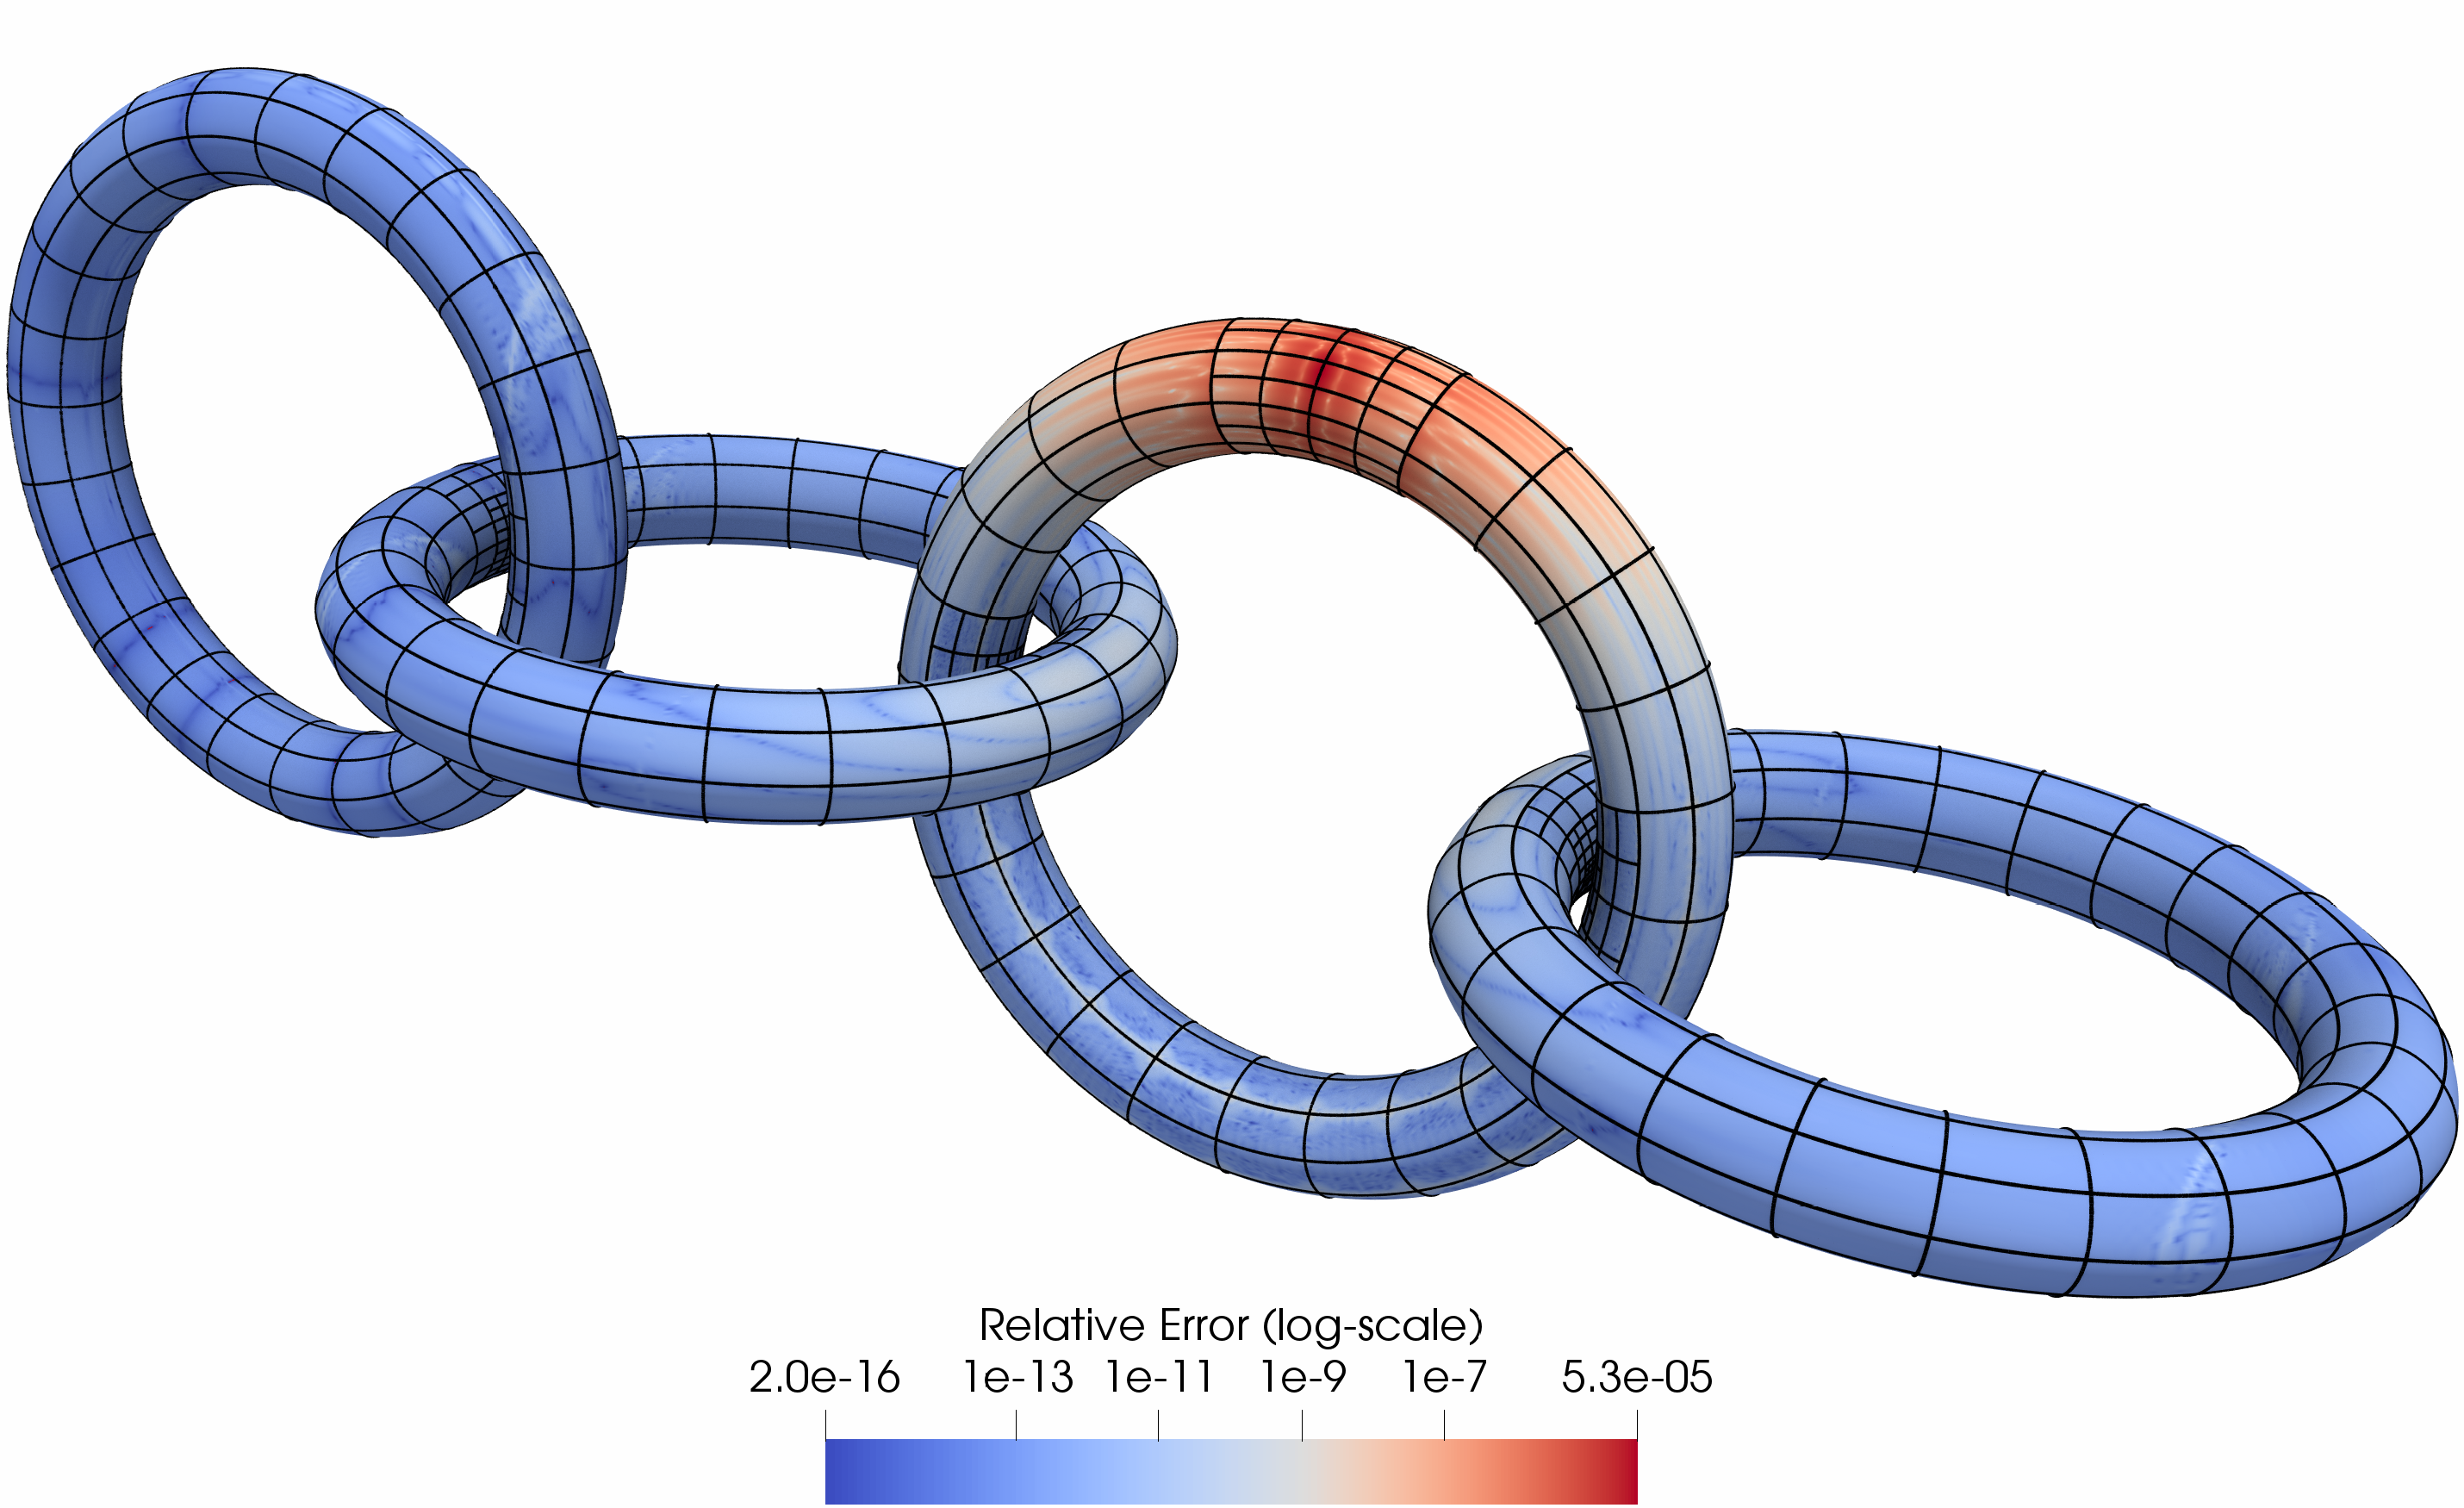
\includegraphics[width=\linewidth]{figs/interlocking_torus_error.png}
  \end{minipage}\hfill
  \begin{minipage}{.35\textwidth}
    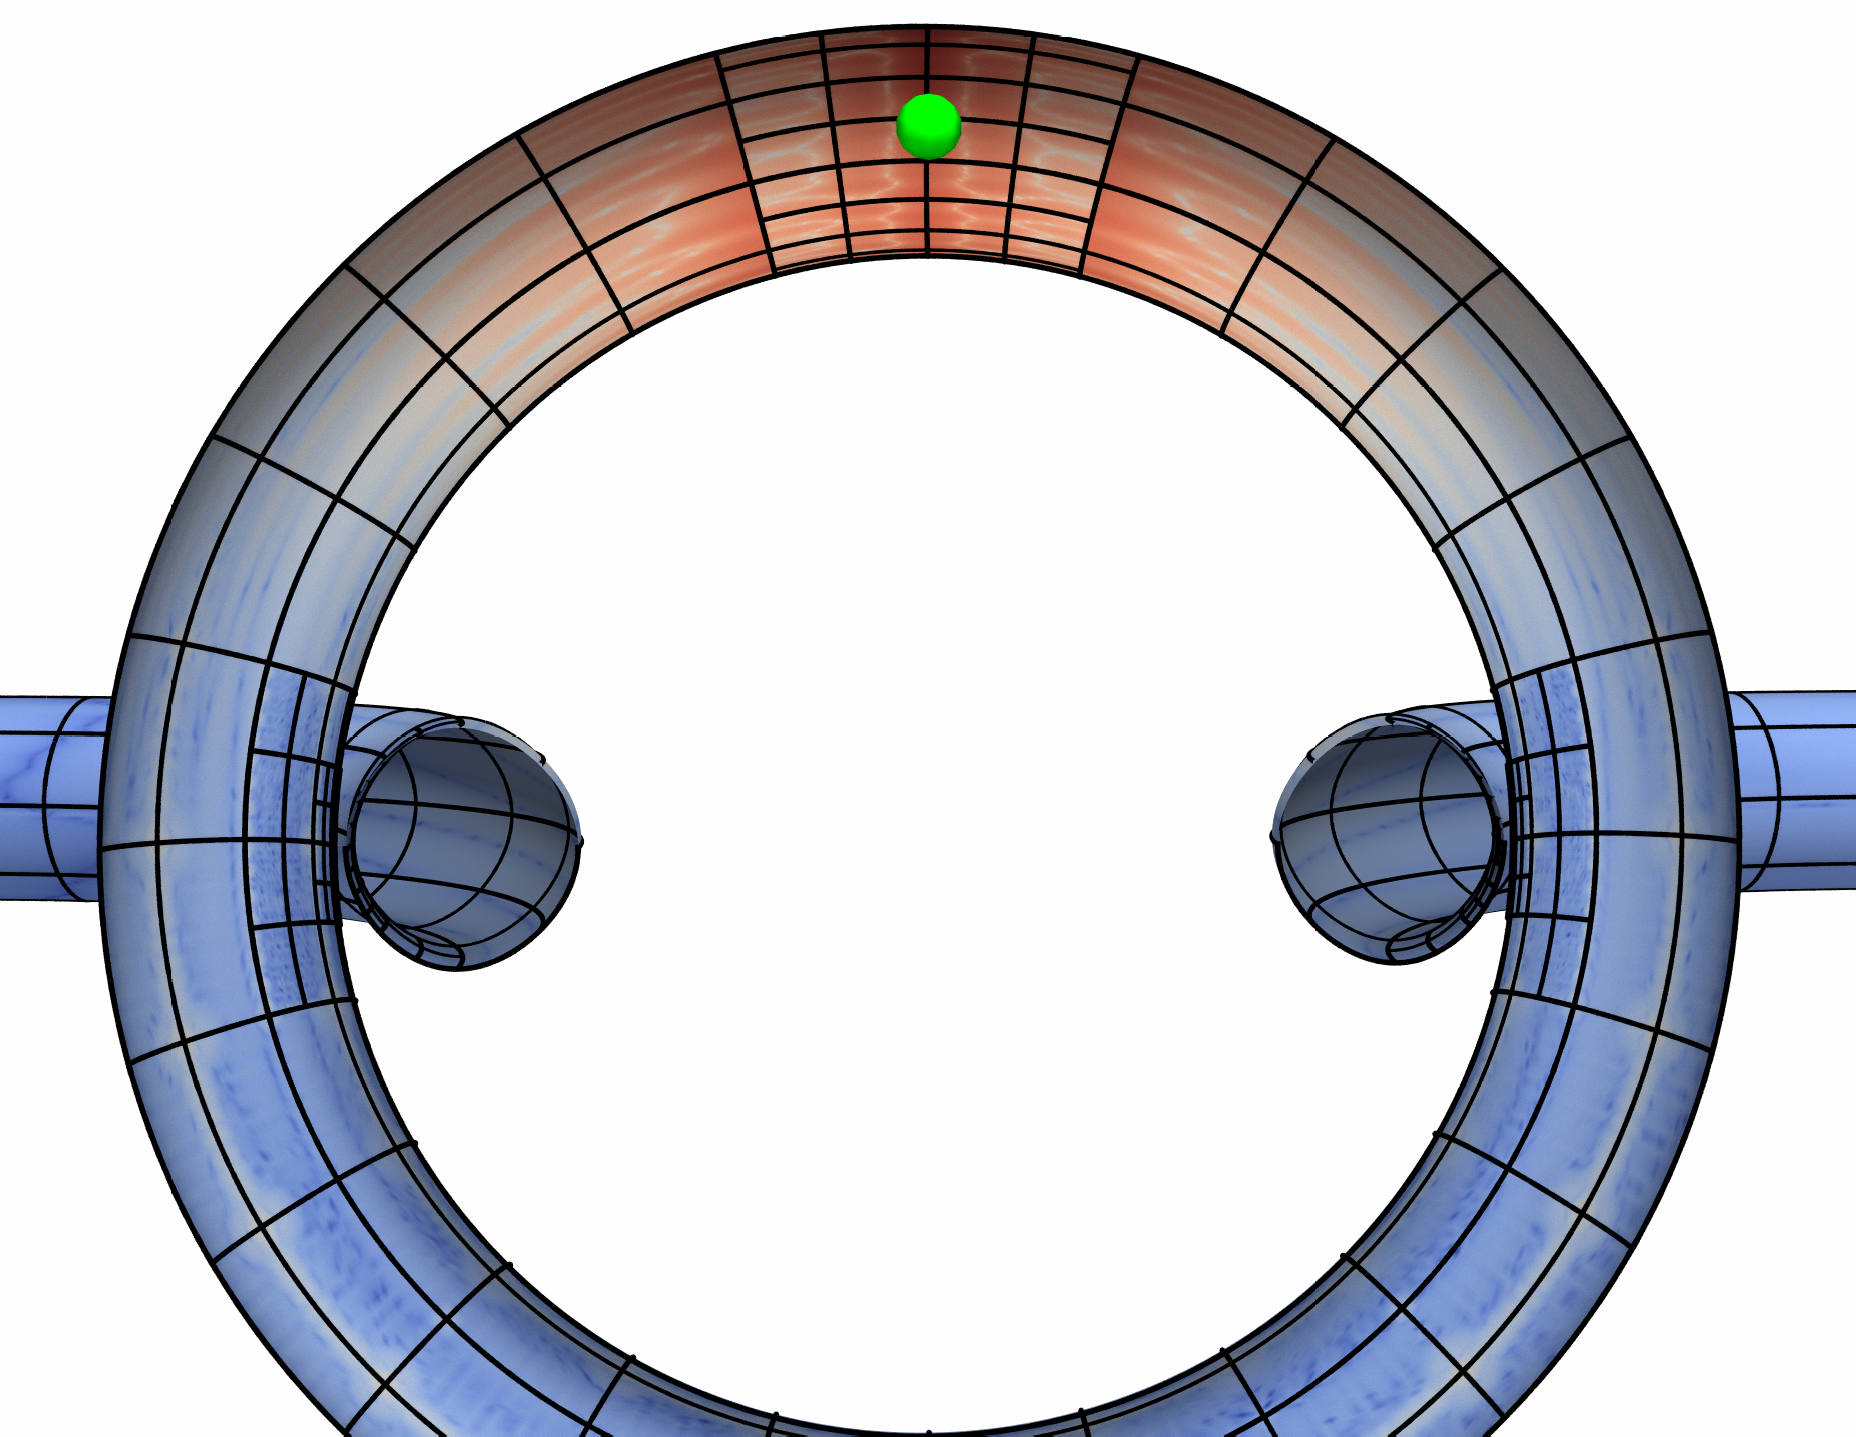
\includegraphics[width=\linewidth]{figs/interlocking_torus_error_cross_section.png}
  \end{minipage}\hfill
  \mcaption{fig:torii}{Absolute error of \gmres solve via \qbkix on interlocking torii}{Left: The admissible set of 1128 patches in $\Pcoarse$ used to solve \cref{eq:int-eq} is shown (black lines denote patch boundaries).
  The point charge generated the boundary condition is located within the second torus from the right. 
    Right: a cross-section of the torii geometry through the $xz$-plane, showing the second torus from the right and the location of the singularity (green point).
}
\end{figure}
Using $a=.1$, $b=.025$, $p=6$ and $q=20$, we achieve a maximum pointwise error of $1.29\times 10^{-5}$. 
\gmres was able to reduce the residual by a factor of $10^{-13}$ over 109 iterations.
There are 288768 quadrature points in the coarse discretization, 18235392 quadrature points in the fine discretization, and 3465216 check points used in the two-sided \qbkix evaluation inside \gmres.
We evaluate the solved density at 451200 points on the boundary with one-sided \qbkix to produce the render in \cref{fig:torii}.
On a machine with two Intel Xeon E-2690v2 3.0GHz \abbrev{CPU}'s, each with 10 cores, and 100 \abbrev{GB} of \abbrev{RAM},
the \gmres solve and interior evaluation required 5.7 hours and can evaluate the singular integral at a rate of 1709 target points per second per core.


\subsection{Solution on complex geometry\label{sec:results-blood-vessel}}

\begin{figure}[!htb]
  \centering
  \setlength\figureheight{1.9in}
  \setlength\figurewidth{2.1in}
  \hfill
  \begin{minipage}{.7\textwidth}
    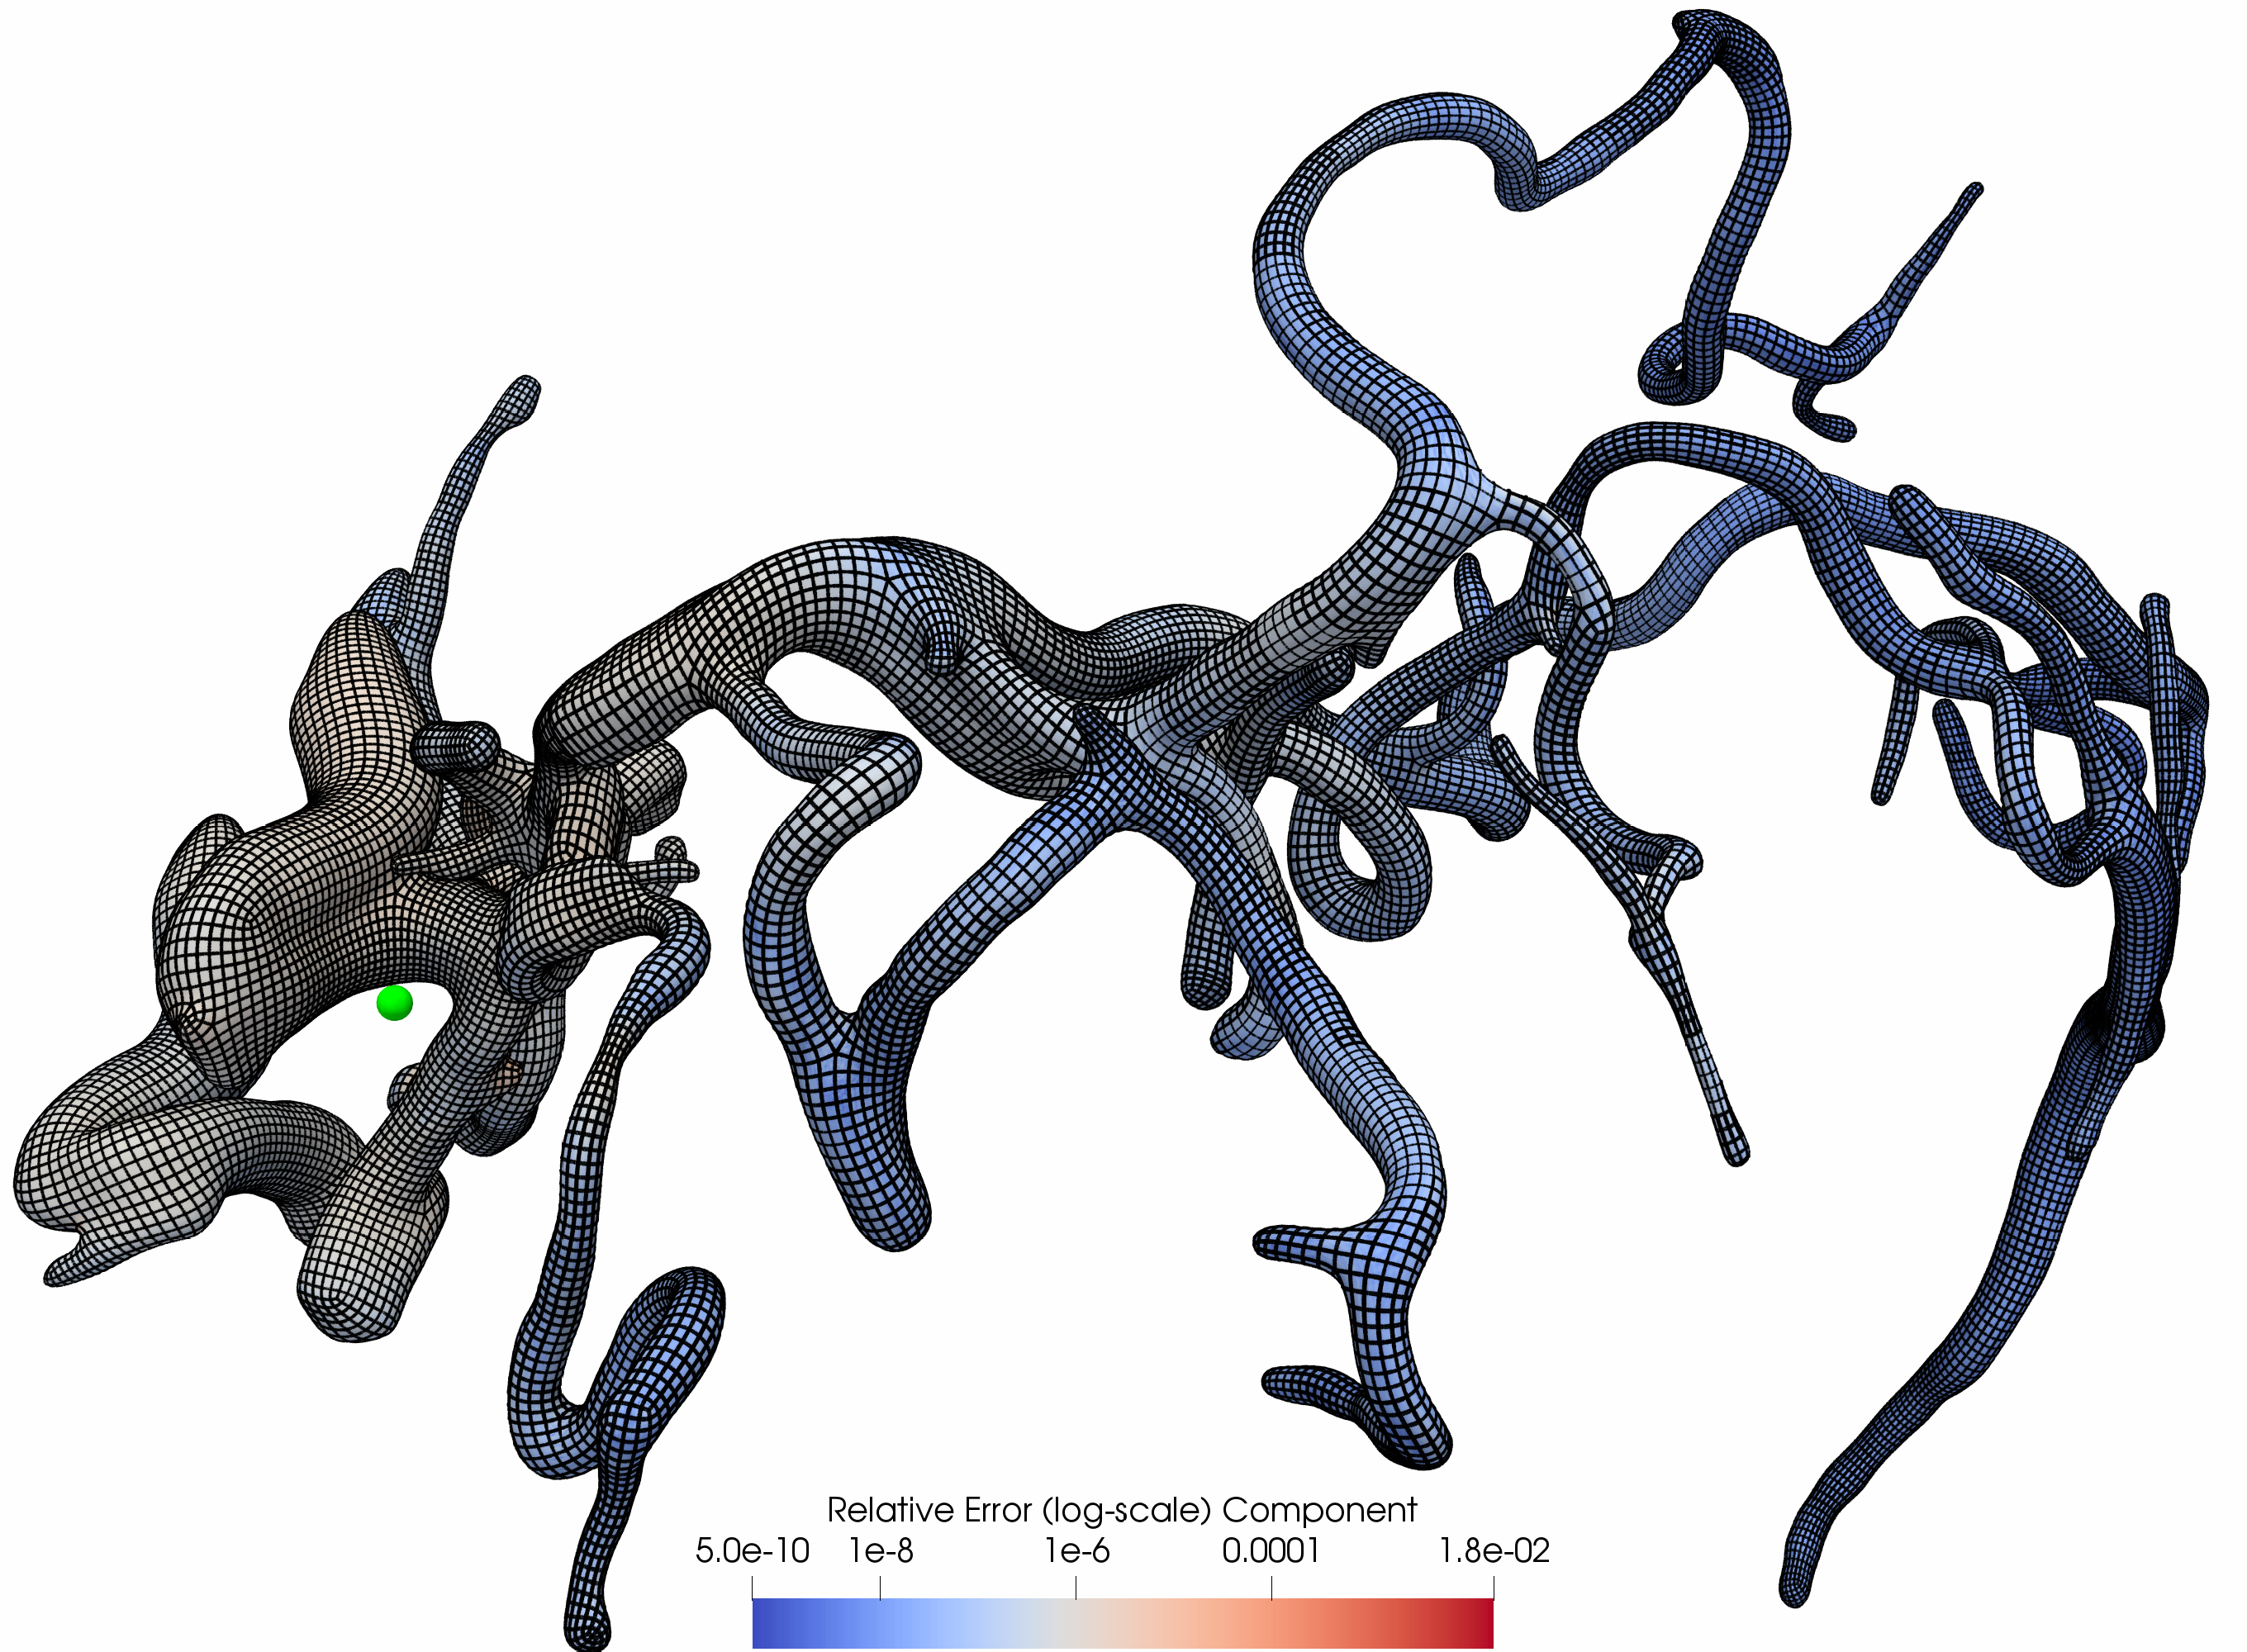
\includegraphics[width=\linewidth]{figs/largest_vessel_section.png}
  \end{minipage}\hfill
  \mcaption{fig:vessel}{Absolute error of \gmres solve via \qbkix on complex blood vessel geometry used in \cite{lu2019scalable}}{The blood vessel uses 40,960 8th order polynomial patches (black edges denote patch boundaries). The geometry is admissible by construction. 
    The point charge is located on left side of the figure (green)}
\end{figure}

We have demonstrated in \cite{lu2019scalable} a parallel implementation of \cref{sec:singular-eval}, applied to simulating red blood cell flows.
The surface geometry of the blood vessel shown in \cref{fig:vessel} is complex, with rapidly varying curvatures and geometric distortions due to singular vertices in the surface mesh.
Since the surface is admissible, we are able to apply parallel \qbkix directly without geometric preprocessing to solve an interior Dirichlet Stokes problem.
We use $a=.125$, $b=.125$, $p=6$ and $q=16$ as simulation parameters.

Using 32 machines each with twenty 2.6 Ghz cores with 100\abbrev{GB} of \abbrev{RAM}, we achieve a maximum pointwise error of $3\times 10^{-6}$ when solving a Stokes problem with constant density. 
We then place a random vector point charge two patch lengths away (relative to the patches in $\Pcoarse$) from the domain boundary (on the left side of \cref{fig:vessel}, solve \cref{eq:int-eq} using two-sided \qbkix, and evaluate the solution on the boundary using one-sided \qbkix.
The absolute error in the $\infty$-norm of the singular evaluation is plotted on the boundary surface.
There are 10,485,760 quadrature points in the coarse discretization, 167,772,160 quadrature points in the fine discretization, and 125,829,120 check points used in the two-sided \qbkix evaluation inside \gmres.
We evaluate the solved density at 209,715,200 points on the boundary with one-sided \qbkix to produce the render in \cref{fig:torii}.
We achieve a maximum pointwise error of $1.8\times 10^{-2}$ and can evaluate the singular integral at rate of 3529 target points per second per core. 
%The \gmres solve with two-sided \qbkix converged to \note[MJM]{X} in \note[MJM]{Y} iterations in \note[MJM]{Z} hours.
\fi
